\documentclass[12pt,a4paper]{ctexart}

\usepackage{geometry}
\usepackage{graphicx}
\usepackage{array}
\usepackage{booktabs}
\usepackage{multirow}
\usepackage{amsmath}
\usepackage{amssymb}
\usepackage{xeCJK}
\usepackage{tikz}
\usepackage{titlesec}

% 页面设置
\geometry{
    top=2.5cm,
    bottom=2.5cm,
    left=2.8cm,
    right=2.8cm
}

% 定义 section* 格式
\titleformat{\section}
  {\zihao{-3}\heiti\bfseries}
  {}
  {0em}
  {}
\titlespacing*{\section}{0pt}{0.5cm}{0.3cm}  % 左缩进、上间距、下间距


% 取消页码（封面）
\pagestyle{empty}

% 定义等长下划线命令（固定宽度 6.5cm，左对齐）
\newcommand{\infofill}[1]{{\zihao{4}\songti\underline{\makebox[6.5cm][c]{#1}}}}

% 定义内容区块命令
\newcommand{\reportsection}[2]{%
    \noindent{\zihao{-3}\heiti\bfseries #1（#2分）}
    \vspace{0.3cm}
    
    \noindent\rule{\textwidth}{0.4pt}
    \vspace{6cm}
}

% 设置中文字体
\setCJKmainfont{SimSun}  % 宋体，可根据系统改为 Noto Serif CJK SC 等

\begin{document}
% ==================== 封面页 ====================
\begin{titlepage}
    \centering
    \vspace*{1.5cm}
    % 校徽占位（正方形示例图）
    
\includegraphics[width=5cm,height=5cm]{images/image-2026-09-07-14-57-04.png}
    
    \vspace{1.8cm}
    
    % 中山大学
    {\zihao{1}\heiti\bfseries 中山大学}
    
    \vspace{0.9cm}
    
    % 微电子科学与技术学院
    {\zihao{2}\heiti 微电子科学与技术学院}
    
    \vspace{0.9cm}
    
    % 课程名称
    {\zihao{2}\heiti 《集成电路元器件特性表征实验》}
    
    \vspace{0.9cm}
    
    % 实验报告
    {\zihao{1}\heiti\bfseries 实验报告}
    
    \vspace{3cm}
    
    % 信息表格
    

    % 信息表格（无任何框线，无横线，无竖线）
    \begin{tabular}{@{}>{\zihao{4}\heiti}r @{\hspace{1.2em}} l@{}}
        实验主题      & \infofill{器件的阻抗特性分析}        \\[0.8cm]
        姓\quad\quad 名 & \infofill{徐睿琳}   \\[0.8cm]
        学\quad\quad 号 & \infofill{23342107} \\[0.8cm]
        实验日期      & \infofill{\today}   \\[0.8cm]
    \end{tabular}
    
    \vfill
\end{titlepage}

% ==================== 内容页 ====================
\newpage
\pagestyle{plain}
\setcounter{page}{2}

\section*{实验目的（5分）}

\begin{enumerate}
    \item 掌握无源线性网络复阻抗 $Z(\omega)=Z'(\omega)+\mathrm{j}Z''(\omega)$ 的频率响应特性，理解电阻、电容、电感及其寄生参数在阻抗谱中的表现，建立 Nyquist 图与 Bode 图的基本原理与对应关系。
    \item 掌握宽频阻抗测试方法：理解小信号正弦激励与对数扫频的必要性，熟悉 LCR 数字电桥的开路/短路补偿及四端接线操作，能够正确采集 $|Z|$、相位 $\varphi$ 及实部、虚部数据。
    \item 掌握基于 ZView 的等效电路建模与拟合方法：依据实测阻抗谱判别电路拓扑结构，拟合提取 $R$、$C$、$L$ 等元件参数，实现由频响数据反演器件物理参数的表征能力。
\end{enumerate}

\section*{实验原理（10分）}

\subsection*{1. 复阻抗与理想元件}
正弦小信号激励下，被测网络的阻抗定义为频率响应函数
\begin{equation}
    Z(\omega)=\frac{\widetilde{V}(\omega)}{\widetilde{I}(\omega)}=Z'(\omega)+\mathrm{j}Z''(\omega)=R+\mathrm{j}X,
    \qquad
    Y(\omega)=\frac{1}{Z(\omega)}=G+\mathrm{j}B .
\end{equation}
实部 $Z'$ 表征耗能与欧姆损耗，虚部 $Z''$ 表征储能与电抗性质（$Z''<0$ 容性、$Z''>0$ 感性）。理想元件的阻抗为
\begin{equation}
    Z_R=R,\qquad Z_C=\frac{1}{\mathrm{j}\omega C}=-\frac{\mathrm{j}}{\omega C},\qquad Z_L=\mathrm{j}\omega L .
\end{equation}

\subsection*{2. 五种无源等效电路的阻抗}

\begin{table}[h]
\centering\footnotesize
\setlength{\tabcolsep}{4pt}
\begin{tabular}{@{}p{2.4cm}|p{5.0cm}|p{5.6cm}@{}}
\hline
拓扑 & 阻抗表达式 $Z(\omega)$ & 频谱特征 \\
\hline
R--C 串联 & $R+\displaystyle\frac{1}{\mathrm{j}\omega C}$ & Nyquist 为 $\mathrm{Re}\,Z=R$ 竖直线；$\varphi:-90^\circ\to0^\circ$ \\
R--C 并联 & $\displaystyle\frac{R}{1+\mathrm{j}\omega R C}$ & 半圆，圆心 $(R/2,0)$、半径 $R/2$，顶点 $\omega_0=1/RC$ \\
(R$\parallel$C)+L & $\mathrm{j}\omega L+\displaystyle\frac{R}{1+\mathrm{j}\omega R C}$ & 低频容性半圆，高频 $\omega L$ 主导进入第四象限 \\
(RC)+(RC) 串联 & $\displaystyle\frac{R_1}{1+\mathrm{j}\omega R_1C_1}+\displaystyle\frac{R_2}{1+\mathrm{j}\omega R_2C_2}$ & 双时间常数，Nyquist 呈两个分离半圆 \\
(R+L)$\parallel$C & $\displaystyle\frac{R+\mathrm{j}\omega L}{1+\mathrm{j}\omega C(R+\mathrm{j}\omega L)}$ & 低频感性、高频容性，$\omega_0\approx1/\sqrt{LC}$ 处并联谐振、$|Z|$ 取极大 \\
\hline
\end{tabular}
\end{table}

\subsection*{3. Bode 图与 Nyquist 图}
Bode 图以 $\lg f$ 为横轴、$|Z|$ 与相位 $\varphi$ 为双纵轴：容性段斜率 $-20\,\mathrm{dB/dec}$，感性段 $+20\,\mathrm{dB/dec}$，转折频率直接给出时间常数 $\tau=1/\omega_0$。Nyquist 图以 $Z'$ 为横轴、$-Z''$ 为纵轴：半圆直径给出电阻值，顶点频率给出 $\tau$，圆弧数目反映弛豫过程个数，轨迹落入第四象限表明存在电感。

\subsection*{4. 寄生参数与等效电路拟合}
实际电阻含引线电感与分布电容，电容含等效串联电阻 ESR、等效串联电感 ESL 及泄漏电阻，电感含直流电阻 DCR 与匝间寄生电容。故实测谱偏离理想模型，须依据实测拓扑在 ZView 中建立含寄生项的等效电路，以非线性最小二乘法拟合提取各元件数值。

\section*{实验设备和步骤（5分）}

\subsection*{1. 实验设备}
同惠 TH2840B 精密 LCR 数字电桥（$20\,\mathrm{Hz}\sim2\,\mathrm{MHz}$）、TH300E 测试夹具、无源元件盲盒（五种待测拓扑）、四端测试电缆、ZView 阻抗分析软件。

\subsection*{2. 实验步骤}
\begin{enumerate}
    \item 开机预热：将 TH300E 电源开关拨至 ON，仪器自检后待机。
    \item 夹具连接：按四端法将测试夹具接入 TH2840B 的 Hc/Hp/Lp/Lc 端，夹具正极接盲盒 High 端，负极接 Low 端，注意插槽极性。
    \item 参数设定：$20\,\mathrm{Hz}\sim2\,\mathrm{MHz}$ 对数扫频，正弦小信号激励（$1\,\mathrm{V}$ 或按仪器默认），每频点取平均以抑制噪声。
    \item 补偿校准：依次执行开路补偿与短路补偿，消除夹具及电缆的并联寄生电容与串联残余阻抗。
    \item 数据采集：启动扫描，记录各频点的 $|Z|$、$\varphi$、$Z'$（RS）、$Z''$（XS）并导出数据文件。
    \item 更换盲盒，重复步骤 2--5，完成五种拓扑的全部测量。
    \item 数据导入 ZView，按实测拓扑建立等效电路模型，设定初值后作非线性最小二乘拟合，提取各元件参数。
\end{enumerate}

\subsection*{3. 注意事项}
\begin{itemize}
    \item 施加偏置时禁止触摸电极，夹具插入须核对极性，避免短路或损坏盲盒。
    \item 高频段注意引线电感与电磁耦合，低频段注意测量时间与温度漂移。
    \item 全程采用小信号激励，确保器件工作于线性区，避免发热引起不可逆变化。
\end{itemize}

\section*{实验数据分析（50分）}

\subsection*{4.1 k1 数据组}

\subsubsection*{（1）数据预处理与拓扑判别}
k1 样品标称为 $R=1\,\mathrm{k}\Omega$（$\pm1\%$）与 $C=100\,\mathrm{nF}$ 串联。实测数据共 801 个频点，覆盖 $20\,\mathrm{Hz}\sim500\,\mathrm{kHz}$，含 $Z'$、$Z''$、$\theta$ 与 $D$，按
\begin{equation}
    |Z|=\sqrt{Z'^2+Z''^2},\qquad \theta=\arctan\frac{Z''}{Z'},\qquad C_{\mathrm{eff}}=-\frac{1}{\omega Z''}
\end{equation}
复算一致性后用于建模。

由图 \ref{fig:k1_bode}、\ref{fig:k1_zy}：$f\ll f_0$ 时 $|Z|$ 以 $-20\,\mathrm{dB/dec}$ 上升、$\theta\to-90^\circ$；$f\gg f_0$ 时 $|Z|$ 趋于平台、$\theta\to0^\circ$。图 \ref{fig:k1_nyq} 中轨迹为 $Z'\approx R$ 的近似竖直线，半圆弧特征缺失。全频段 $Z''<0$，无第四象限数据点，据此判定该样品为 \textbf{R--C 串联}结构且不含可辨识电感。

\subsection*{（2）等效电路建模与拟合}
取串联模型 $Z(\omega)=R-\mathrm{j}/(\omega C)$，在 ZView 中以比例权重（$\Delta Z/|Z|$）对实部、虚部作复数非线性最小二乘拟合：
\begin{equation}
    \min_{R,C}\sum_{i=1}^{N}\left[\left(\frac{Z'_i-Z'_{\mathrm{mod}}}{|Z_i|}\right)^2+\left(\frac{Z''_i-Z''_{\mathrm{mod}}}{|Z_i|}\right)^2\right].
\end{equation}
为检验寄生效应，另设 R--L--C 串联与 $R$--CPE（$Z=R+1/[Q(\mathrm{j}\omega)^n]$）两个对照模型。

\begin{figure}[htbp]
\centering
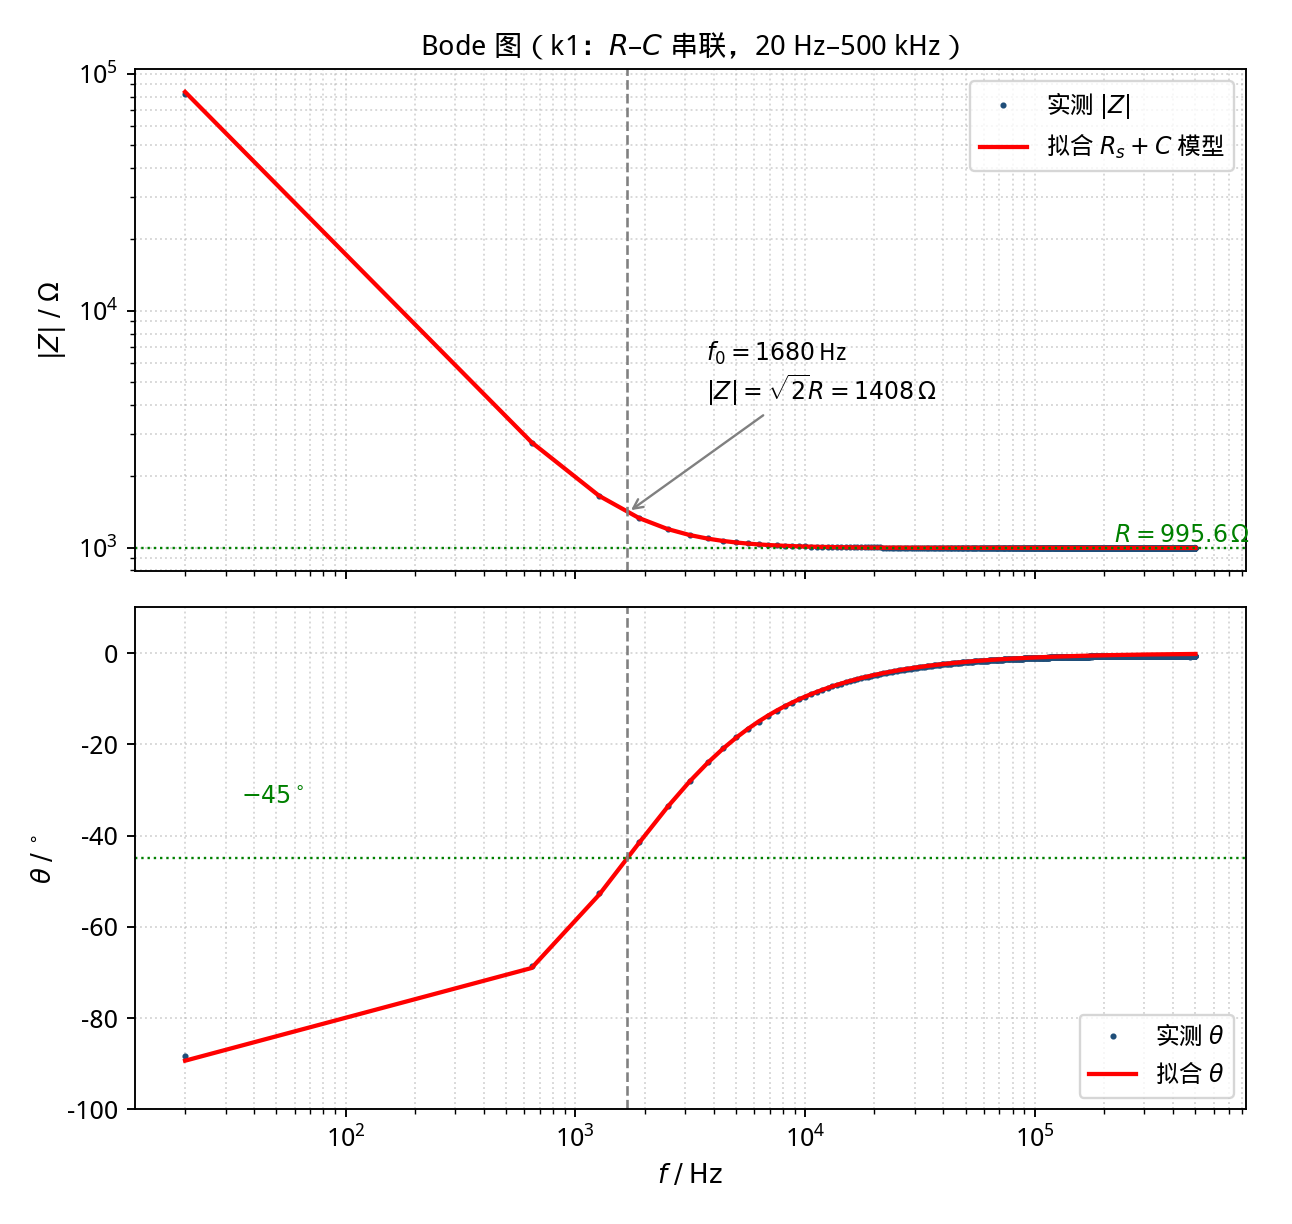
\includegraphics[width=0.82\textwidth]{images/image-2026-10-07-19-25-56.png}
\caption{k1 的 Bode 图（$|Z|$、$\theta$ 与频率），散点为实测，实线为 $R_s$--$C$ 模型拟合结果。}
\label{fig:k1_bode}
\end{figure}

\begin{figure}[htbp]
\centering
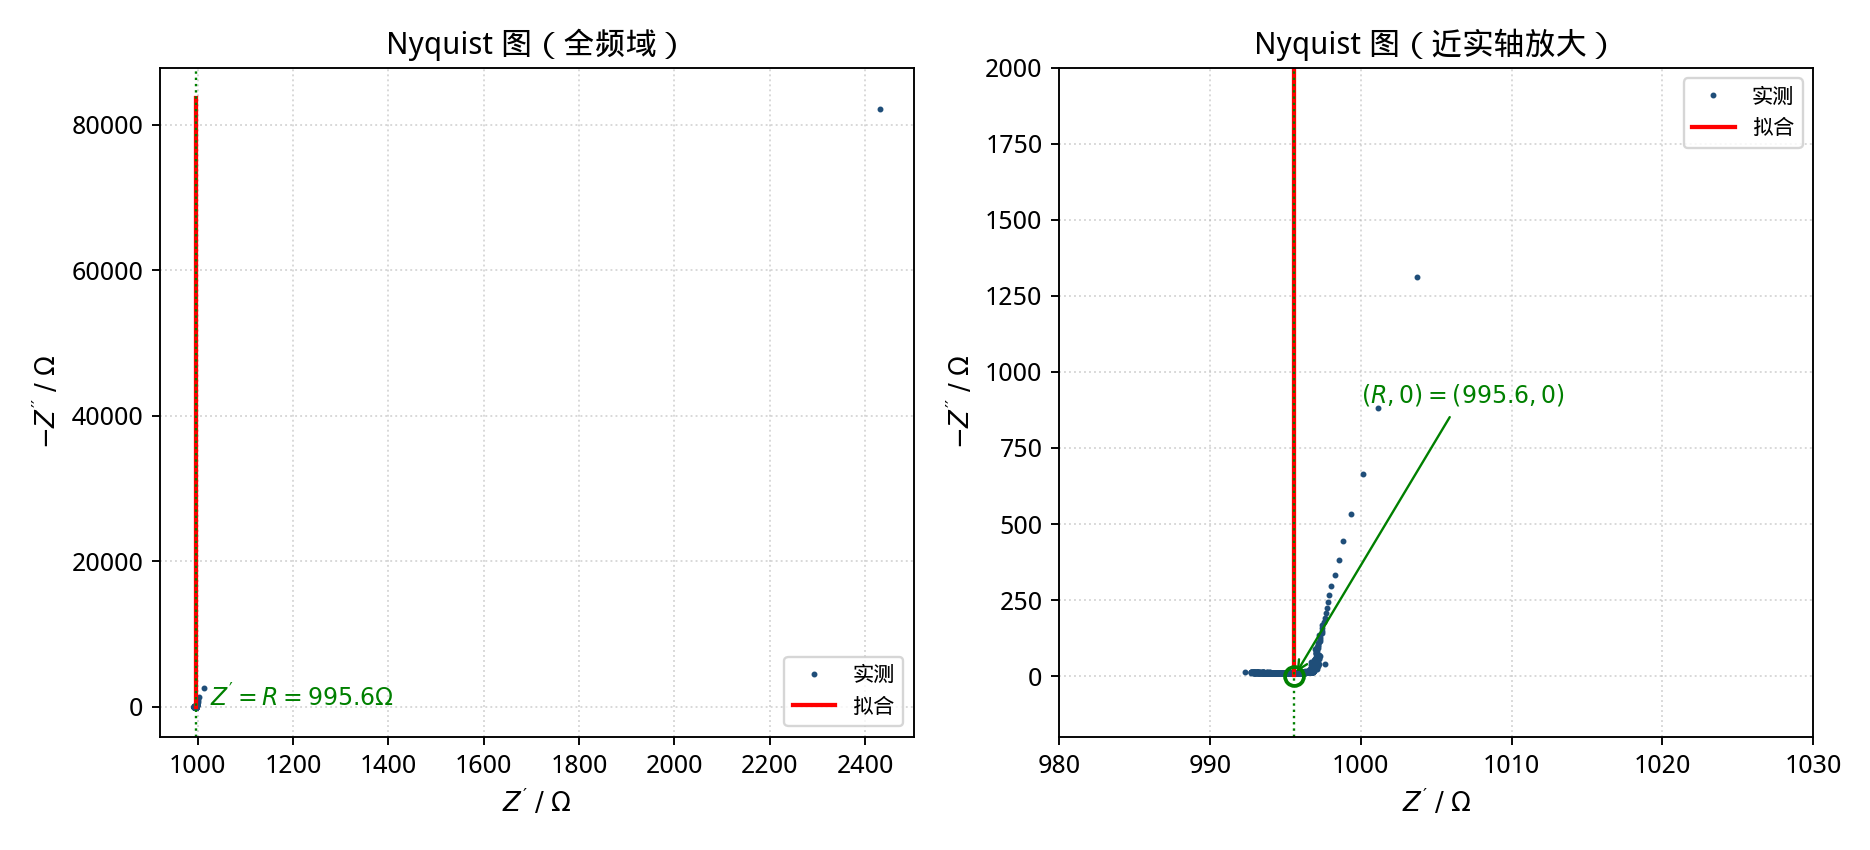
\includegraphics[width=0.98\textwidth]{images/image-2026-10-07-19-26-24.png}
\caption{k1 的 Nyquist 图：左为全频域，呈 $Z'=R$ 竖直线；右为近实轴放大，圆弧与实轴交点即串联电阻 $R$。}
\label{fig:k1_nyq}
\end{figure}

\subsection*{（3）拟合结果与参数提取}
\begin{table}[htbp]
\centering\small
\begin{tabular}{l|c|c|c}
\hline
参数 & 拟合值 & 标称值 & 相对偏差 \\
\hline
$R$ & $995.60\pm0.20\ \Omega$ & $1\,\mathrm{k}\Omega\ (\pm1\%)$ & $-0.44\%$ \\
$C$ & $95.13\pm0.40\ \mathrm{nF}$ & $100\,\mathrm{nF}$ & $-4.87\%$ \\
$\tau=RC$ & $94.71\ \mu\mathrm{s}$ & $100\ \mu\mathrm{s}$ & $-5.29\%$ \\
$f_0=1/(2\pi RC)$ & $1.680\ \mathrm{kHz}$ & $1.592\ \mathrm{kHz}$ & $+5.6\%$ \\
\hline
\end{tabular}
\end{table}

主要判据：$\theta=-45^\circ$ 实测出现在 $1.664\ \mathrm{kHz}$，与拟合 $f_0=1.680\ \mathrm{kHz}$ 相差 $1\%$；$20\ \mathrm{Hz}$ 处 $|Z|=82.13\ \mathrm{k}\Omega$、$\theta=-88.30^\circ$，$470.6\ \mathrm{kHz}$ 处 $|Z|$ 取极小 $992.4\ \Omega\approx R$，均符合 R--C 串联预期。$R$ 落在 $990\sim1010\ \Omega$ 容差带内，$C$ 偏差在常见 $\pm5\%$ 容差内，二者一致性良好。

对照模型：R--L--C 拟合给出 $L=-2.90\ \mu\mathrm{H}$（负值不具物理意义），说明引入电感项仅为吸收高频残差，不能改善模型真实性，反证样品无电感；$R$--CPE 拟合 $n=0.991\sim0.994$，逼近 1，表明电容弥散效应微弱、理想电容近似成立。

\begin{figure}[htbp]
\centering
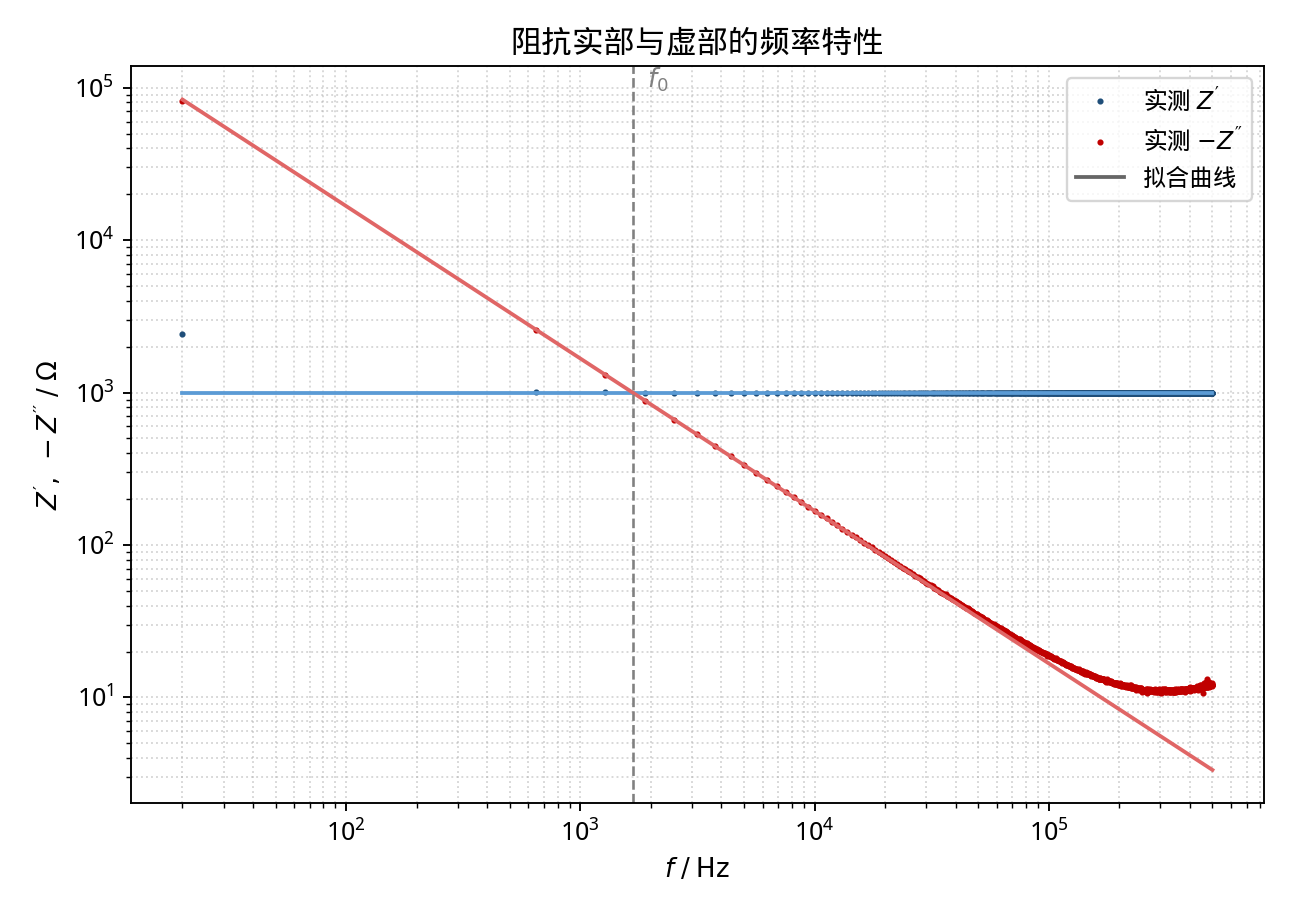
\includegraphics[width=0.82\textwidth]{images/image-2026-10-07-19-26-47.png}
\caption{$Z'$ 与 $-Z''$ 的双对数频率特性，两曲线在 $f_0$ 附近交叉，交叉频率即转折频率。}
\label{fig:k1_zy}
\end{figure}

\subsection*{（4）残差与不确定度分析}
拟合的 $\chi^2=1.52\times10^{-5}$，加权 RMS 残差 $0.39\%$，$Z'$、$Z''$ 的归一化残差随频率分布见图 \ref{fig:k1_res}。

\begin{figure}[htbp]
\centering
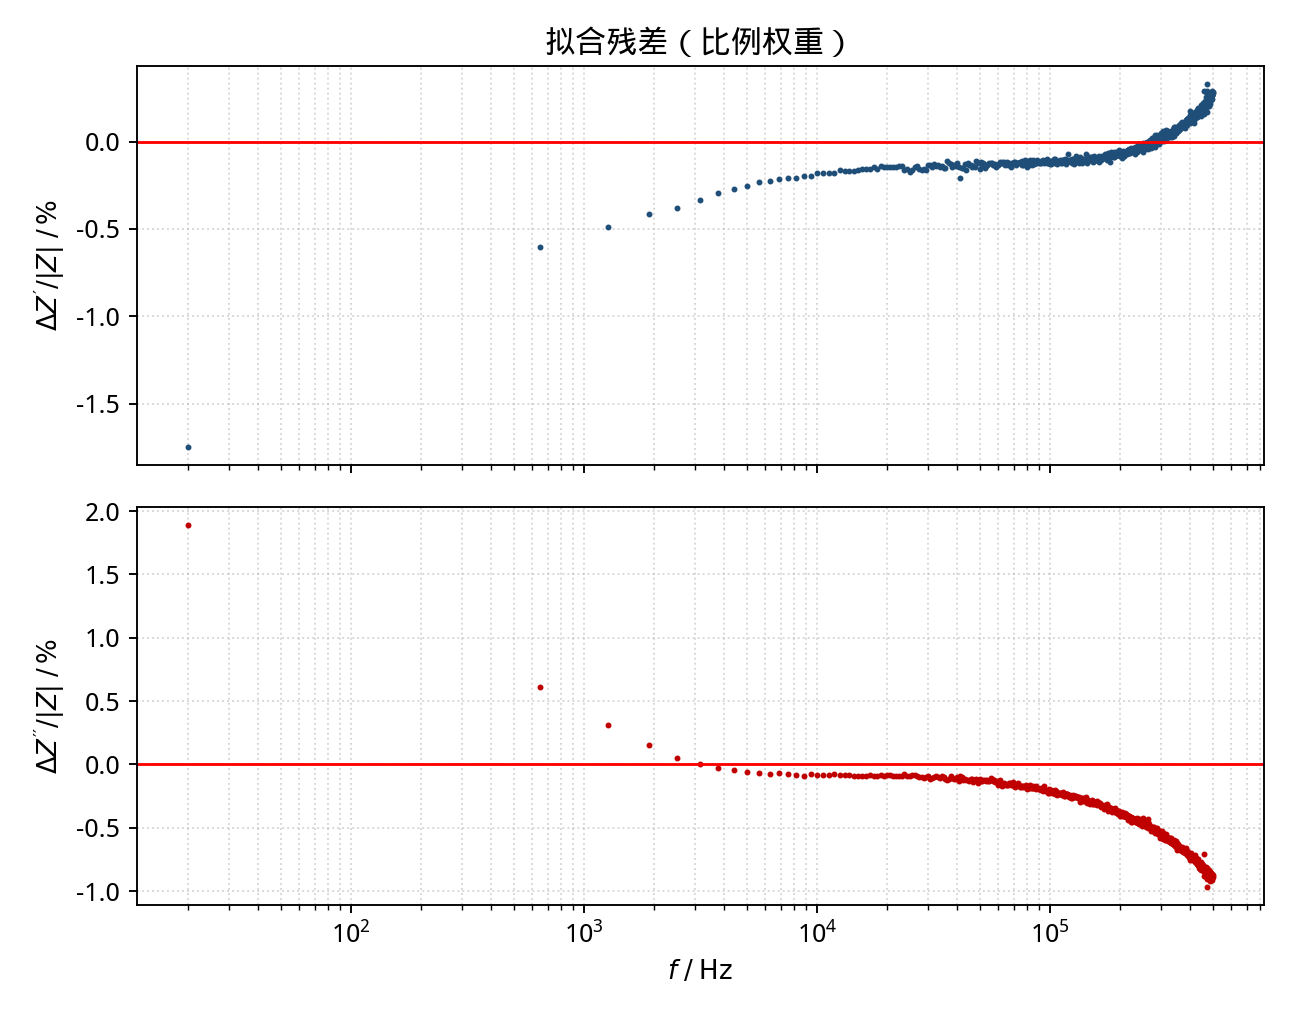
\includegraphics[width=0.82\textwidth]{images/image-2026-10-07-19-27-02.png}
\caption{比例权重下的拟合残差，中频段 $|\Delta Z|/|Z|<0.5\%$，高频端残差显著增大。}
\label{fig:k1_res}
\end{figure}

\begin{itemize}
    \item \textbf{高频段（$f>200\ \mathrm{kHz}$）}：$Z''$ 相对理想 $-1/(\omega C)$ 存在约 $-9\ \Omega$ 系统性偏差（等效为 $-2.9\ \mu\mathrm{H}$ 虚假串联电感，即约 $35\ \mathrm{nF}$ 等效串联电容误差）。源于夹具与电缆的开路残余导纳未完全补偿，以及 LCR 电桥在 $|Z''|/|Z|\sim10^{-3}$ 微相位角下的分辨力限制；图 \ref{fig:k1_ceff} 中 $C_{\mathrm{eff}}$ 在该段明显偏低即为同一效应的表现。剔除该段后拟合为 $R=996.82\ \Omega$、$C=95.43\ \mathrm{nF}$，参数漂移 $<0.3\%$，证明主拟合稳健。
    \item \textbf{最低频点（$20\ \mathrm{Hz}$）}：$Z'=2430.9\ \Omega$ 显著偏离平台值，系该点测量周期长、信噪比低导致的约 $1^\circ$ 相位误差，属异常点；因采用比例权重，其对参数提取的贡献已自动弱化。
    \item \textbf{系统误差}：电阻偏差 $-0.44\%$、电容偏差 $-4.87\%$ 由元件实际容差与夹具残余阻抗共同构成；线性等间隔扫频使 $f_0$ 附近有效频点仅 4 个，是 $f_0$ 不确定度的主要来源。
\end{itemize}

\begin{figure}[htbp]
\centering
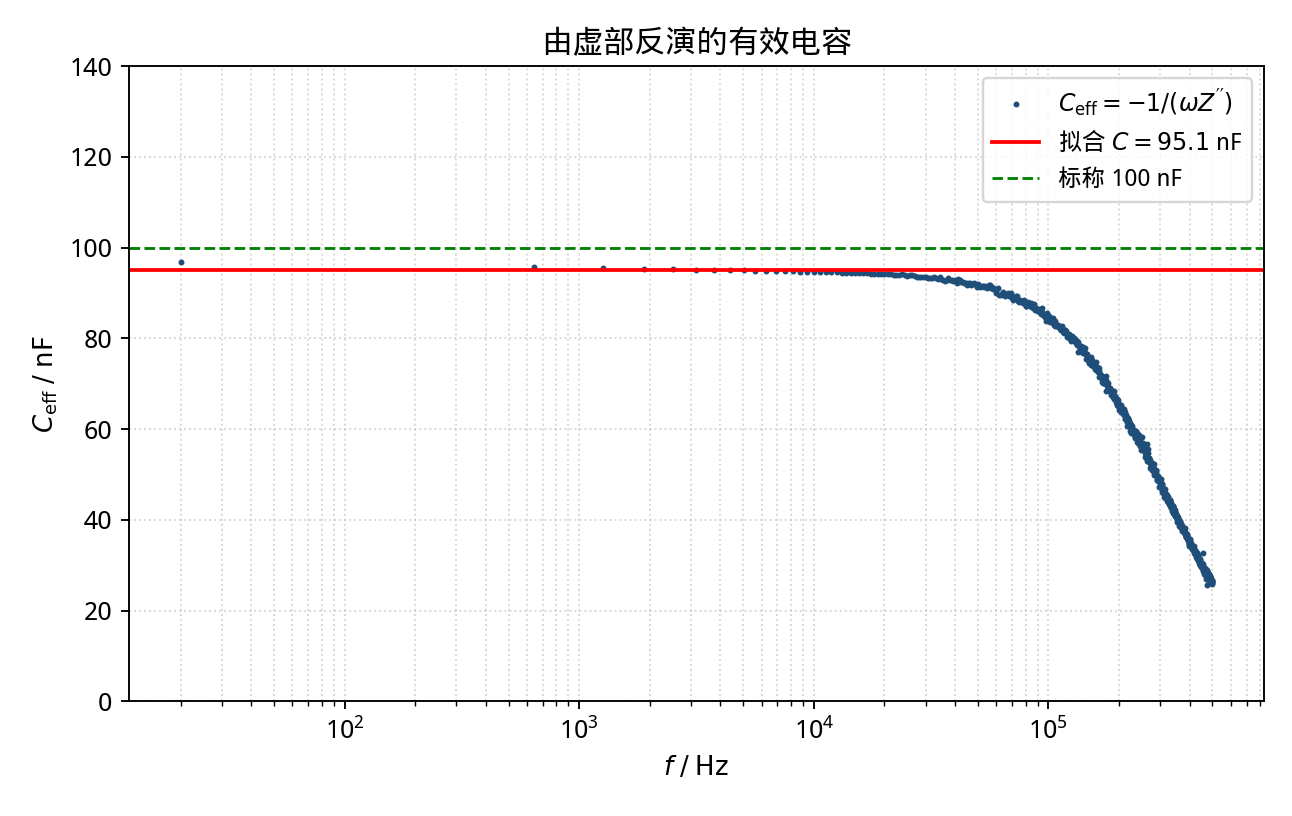
\includegraphics[width=0.78\textwidth]{images/image-2026-10-07-19-27-21.png}
\caption{由 $C_{\mathrm{eff}}=-1/(\omega Z'')$ 反演的表观电容，低频段收敛于拟合值 $95.1\ \mathrm{nF}$。}
\label{fig:k1_ceff}
\end{figure}

\subsection*{（5）结论}
k1 样品的阻抗谱具备单一时间常数、$Z'=R$ 恒定的容性竖直轨迹特征，判定为 R--C 串联结构，不存在可辨识电感。ZView 拟合给出 $R=995.60\ \Omega$、$C=95.13\ \mathrm{nF}$，与标称值偏差分别为 $-0.44\%$ 与 $-4.87\%$，均在元件容差范围内，拟合残差 $0.39\%$，验证了串联网路阻抗模型与参数反演方法的有效性。

\subsection*{4.2 k2 数据组}

\subsubsection*{（1）数据概况与拓扑判别}
本组共 801 个频点，扫频范围 $20\,\mathrm{Hz}\sim100\,\mathrm{kHz}$，频率步进固定 $125\,\mathrm{Hz}$。全频段 $Z''<0$，无第四象限数据点；相位由 $20\,\mathrm{Hz}$ 处的 $-4.91^\circ$ 单调变至 $100\,\mathrm{kHz}$ 处的 $-89.13^\circ$。

图 \ref{fig:k2_nyq} 中 Nyquist 轨迹为位于容性半平面的\textbf{闭合半圆}而非竖直线：低频端收敛于实轴 $Z'\to R$，高频端经顶点回零。此特征是 R--C 并联（$Z=R\parallel 1/(\mathrm{j}\omega C)$）区别于 R--C 串联（$Z'=R$ 恒定竖线）的判据，据此判定 k2 为 R--C 并联结构。

\subsubsection*{（2）等效电路建模}
R--C 并联的理想阻抗为
\begin{equation}
    Z(\omega)=\frac{R}{1+\mathrm{j}\omega R C}=\frac{R}{1+(\omega R C)^2}-\mathrm{j}\frac{\omega R^2 C}{1+(\omega R C)^2},
    \qquad \left(Z'-\frac{R}{2}\right)^2+Z''^2=\left(\frac{R}{2}\right)^2 .
\end{equation}
即在 Nyquist 图上为圆心 $(R/2,0)$、半径 $R/2$ 的半圆，顶点处 $\omega_0RC=1$，$-Z''_{\max}=R/2$。

实测高频端 $Z'$ 未趋于零而收敛于约 $0.3\,\Omega$，且半圆略偏离理想圆，故按 ZView 流程依次建立并比较四个模型：

\begin{equation}
    \begin{array}{l}
        Z_{1}=\frac{1}{\frac{1}{R}+\mathrm{j}\omega C},\qquad
        Z_{2}=R_s+Z_{1},\\[4pt]
        Z_{3}=R_s+\frac{1}{\frac{1}{R}+Q(\mathrm{j}\omega)^{n}},\qquad
        Z_{4}=R_s+\mathrm{j}\omega L+Z_{\mathrm{CPE}} .
    \end{array}
\end{equation}

以比例权重 $\Delta Z/|Z|$ 对实部、虚部同时作复数非线性最小二乘拟合，结果见表 \ref{tab:k2_model}。

\begin{table}[htbp]\centering\small
\begin{tabular}{l|c|c}
\hline
模型 & 拟合参数 & 加权 RMS 残差 \\
\hline
$R\parallel C$ & $R=9703.8\,\Omega,\ C=76.71\,\mathrm{nF}$ & $0.719\%$ \\
$R_s+(R\parallel C)$ & $R=9794.6\,\Omega,\ C=76.71\,\mathrm{nF},\ R_s=0.332\,\Omega$ & $0.306\%$ \\
$R_s+(R\parallel\mathrm{CPE})$ & $R=9931.9\,\Omega,\ Q=79.88\,\mathrm{nF},n=0.9967,\ R_s=0.173\,\Omega$ & $0.125\%$ \\
$R_s+L+(R\parallel\mathrm{CPE})$ & $L=+0.207\,\mu\mathrm{H}$ & $0.068\%$ \\
\hline
\end{tabular}
\end{table}

\begin{figure}[htbp]\centering
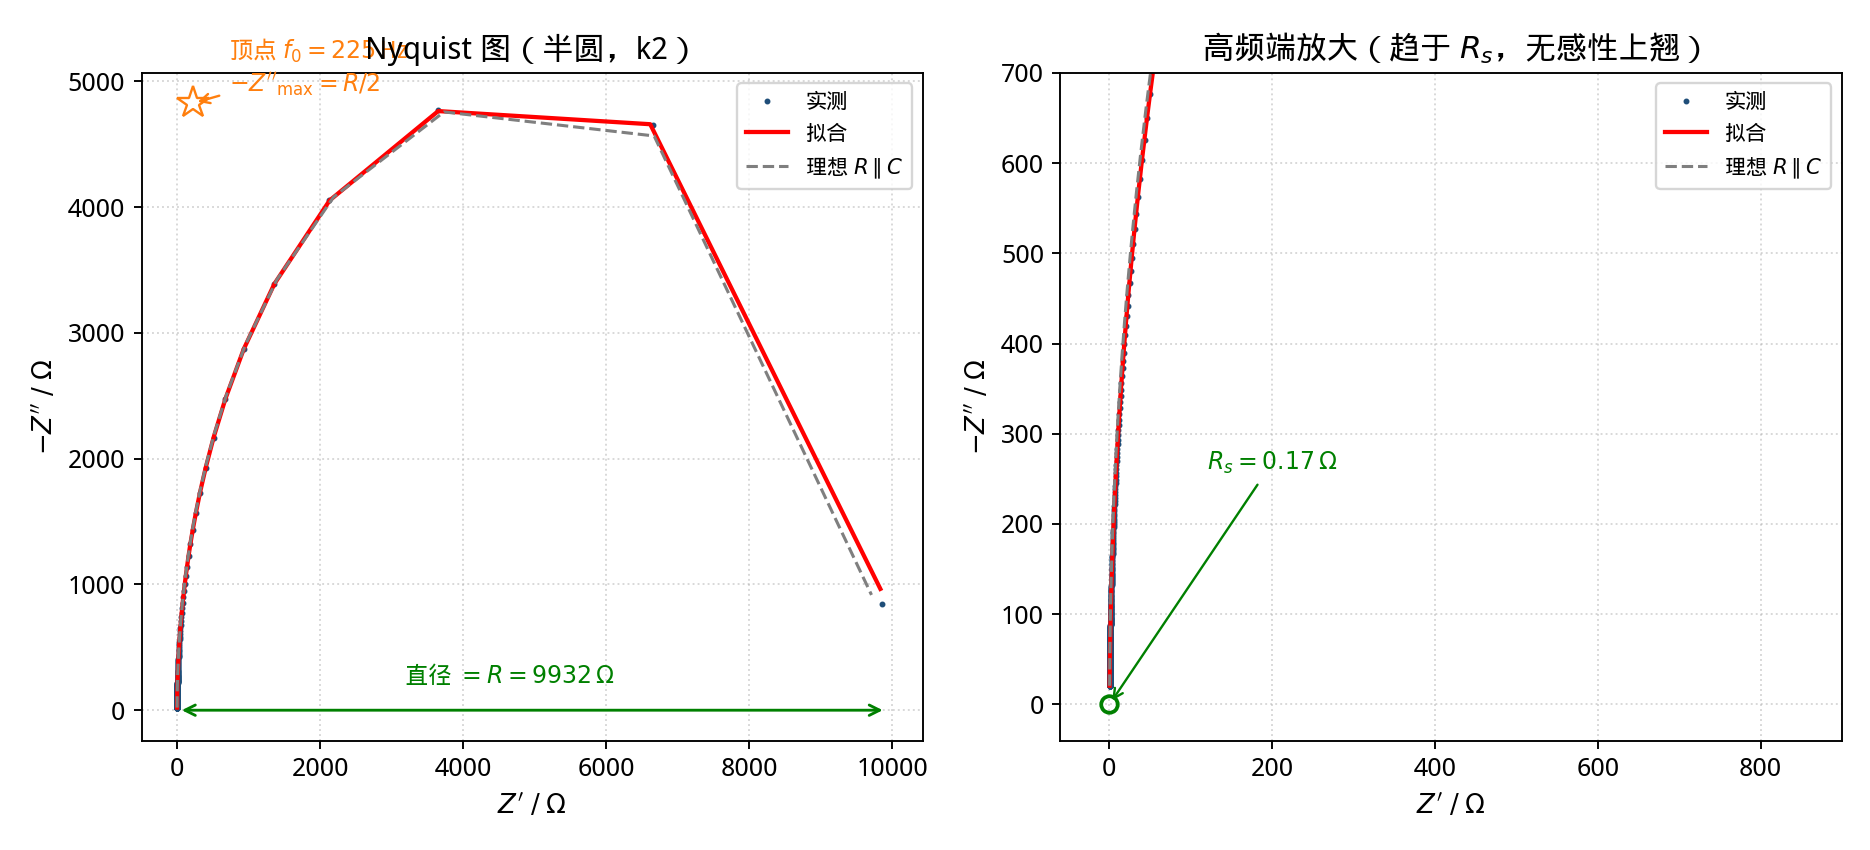
\includegraphics[width=0.98\textwidth]{images/image-2026-10-07-19-43-18.png}
\caption{k2 的 Nyquist 图：左为标准容性半圆（直径即 $R$，顶点对应 $f_0$）；右为高频端放大，轨迹收敛于 $R_s$，无感性上翘。}
\label{fig:k2_nyq}
\end{figure}

\subsubsection*{（3）拟合结果与参数提取}
取模型 $Z_3$ 为最终结果，参数见表 \ref{tab:k2_fit}。CPE 指数 $n=0.9967\pm0.0001$ 极接近 1，说明电容仅有微弱介电弥散，理想电容近似基本成立；串联项 $R_s=0.173\,\Omega$ 为引线、接触与电容 ESR 的合计残余电阻。

\begin{table}[htbp]\centering\small
\begin{tabular}{l|c|c|c}
\hline
参数 & 拟合值 & 标称值 & 相对偏差 \\
\hline
$R$ & $9931.9\pm7.8\,\Omega$ & $10\,\mathrm{k}\Omega\ (\pm1\%,\ 9900\sim10100)$ & $-0.68\%$（合格） \\
$C_{\mathrm{eff}}$ & $78.03\,\mathrm{nF}$ & $82\,\mathrm{nF}$ & $-4.85\%$ \\
$R_s$ & $0.173\pm0.002\,\Omega$ & — & — \\
$n$（CPE） & $0.99673\pm0.00001$ & 1 & $-0.33\%$ \\
\hline
\multicolumn{4}{l}{导出量：$\tau=(RQ)^{1/n}=0.775\,\mathrm{ms}$，$f_0=1/(2\pi\tau)=205.4\,\mathrm{Hz}$，$-Z''_{\max}=R/2=4966\,\Omega$}
\end{tabular}
\end{table}

\begin{figure}[htbp]\centering
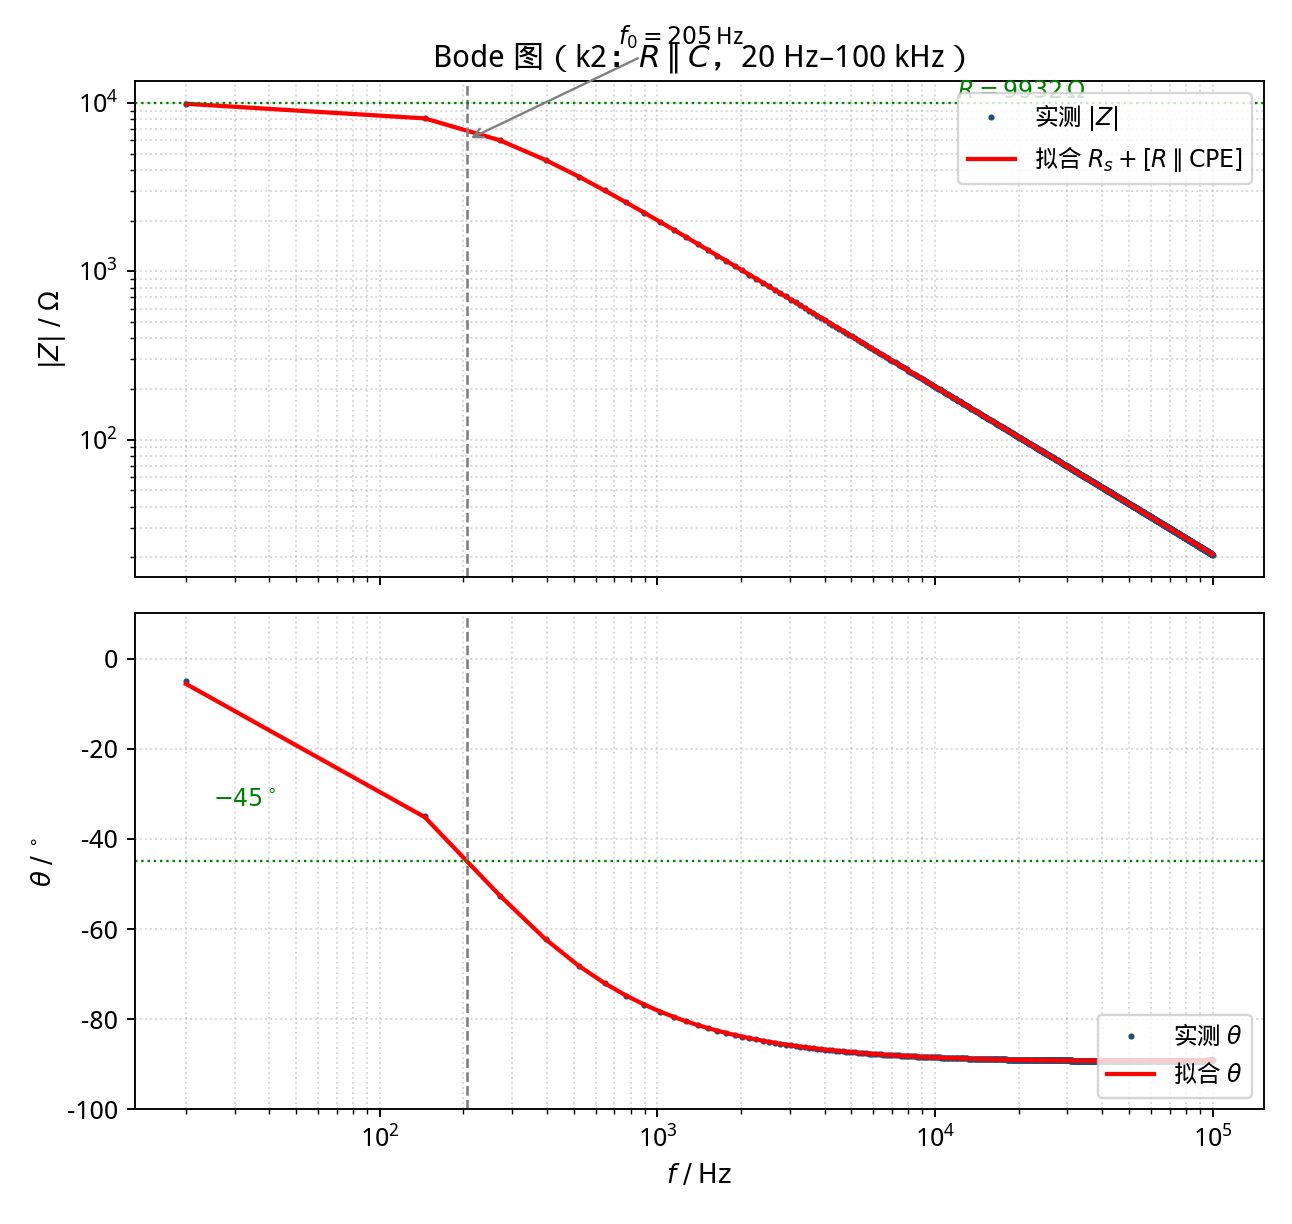
\includegraphics[width=0.82\textwidth]{images/image-2026-10-07-19-43-43.png}
\caption{k2 的 Bode 图：$|Z|$ 低频趋于 $R$ 平台、高频以 $-20\,\mathrm{dB/dec}$ 下降；相位由 $0^\circ$ 过渡至 $-90^\circ$，$f_0$ 处为 $-45^\circ$。}
\label{fig:k2_bode}
\end{figure}

\subsubsection*{（4）独立交叉校验}
将实测阻抗取倒数得导纳 $Y=G+\mathrm{j}B$，对 R--C 并联应有 $1/G\to R$、$B/\omega\to C$ 为常数（图 \ref{fig:k2_adm}）。实测 $1/G$ 在 $20\,\mathrm{Hz}$ 处为 $9924.4\,\Omega$，与拟合 $R=9931.9\,\Omega$ 相差 $0.08\%$；$C_p=B/\omega$ 在 $300\,\mathrm{Hz}\sim100\,\mathrm{kHz}$ 区间稳定于 $76.5\sim77.9\,\mathrm{nF}$，与 $C_{\mathrm{eff}}=78.0\,\mathrm{nF}$ 一致。两种方法独立给出同一结果，证明参数提取可靠。

\begin{figure}[htbp]\centering
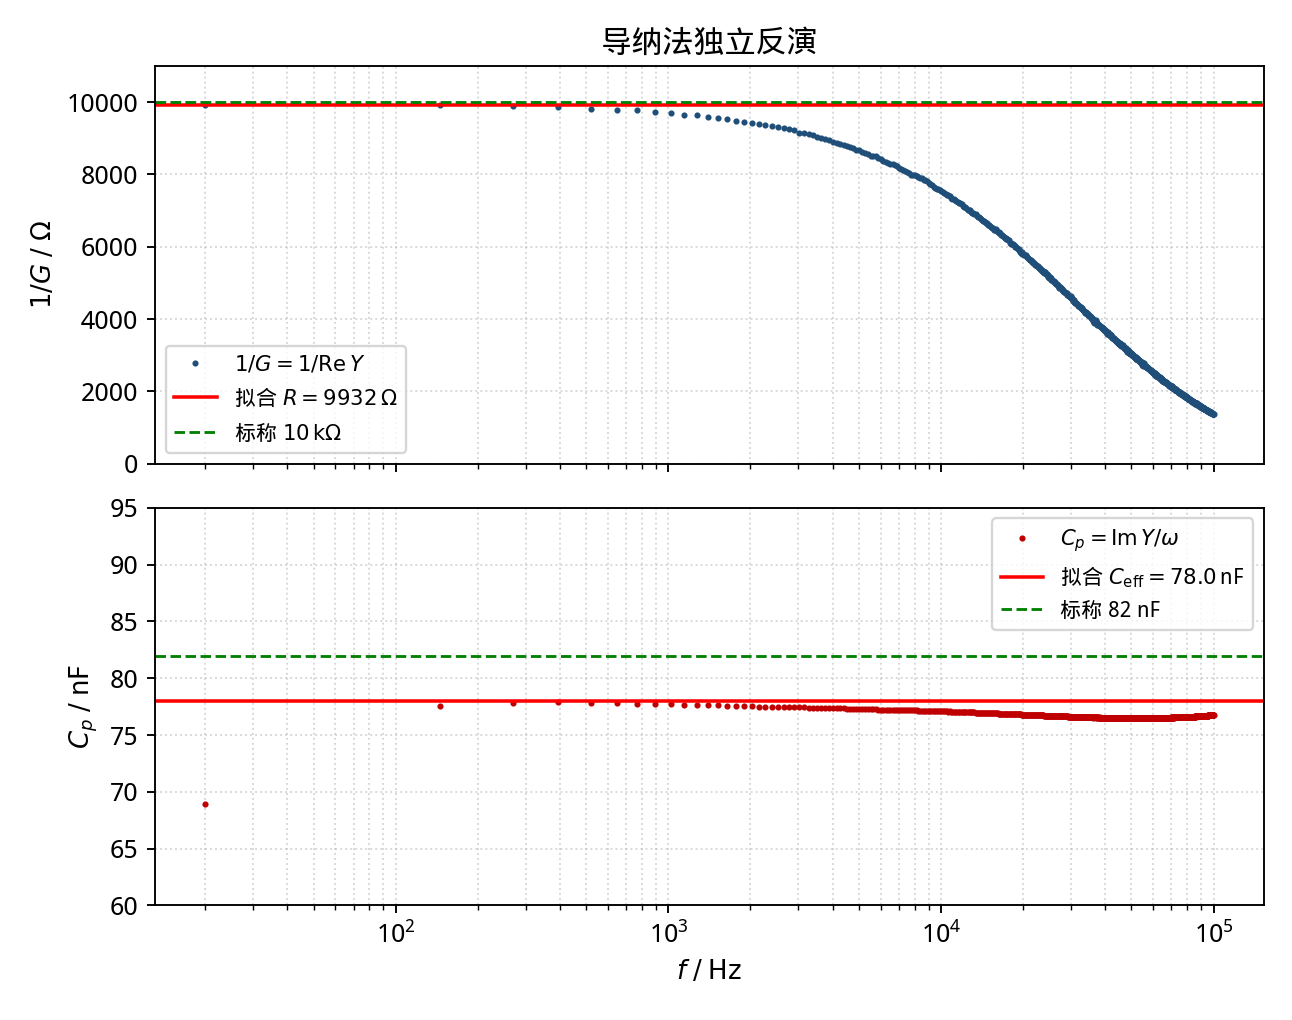
\includegraphics[width=0.82\textwidth]{images/image-2026-10-07-19-44-05.png}
\caption{导纳法独立反演：上图 $1/G$ 在低频收敛于 $R$，下图 $C_p=B/\omega$ 在全频段近于平台。}
\label{fig:k2_adm}
\end{figure}

\begin{figure}[htbp]\centering
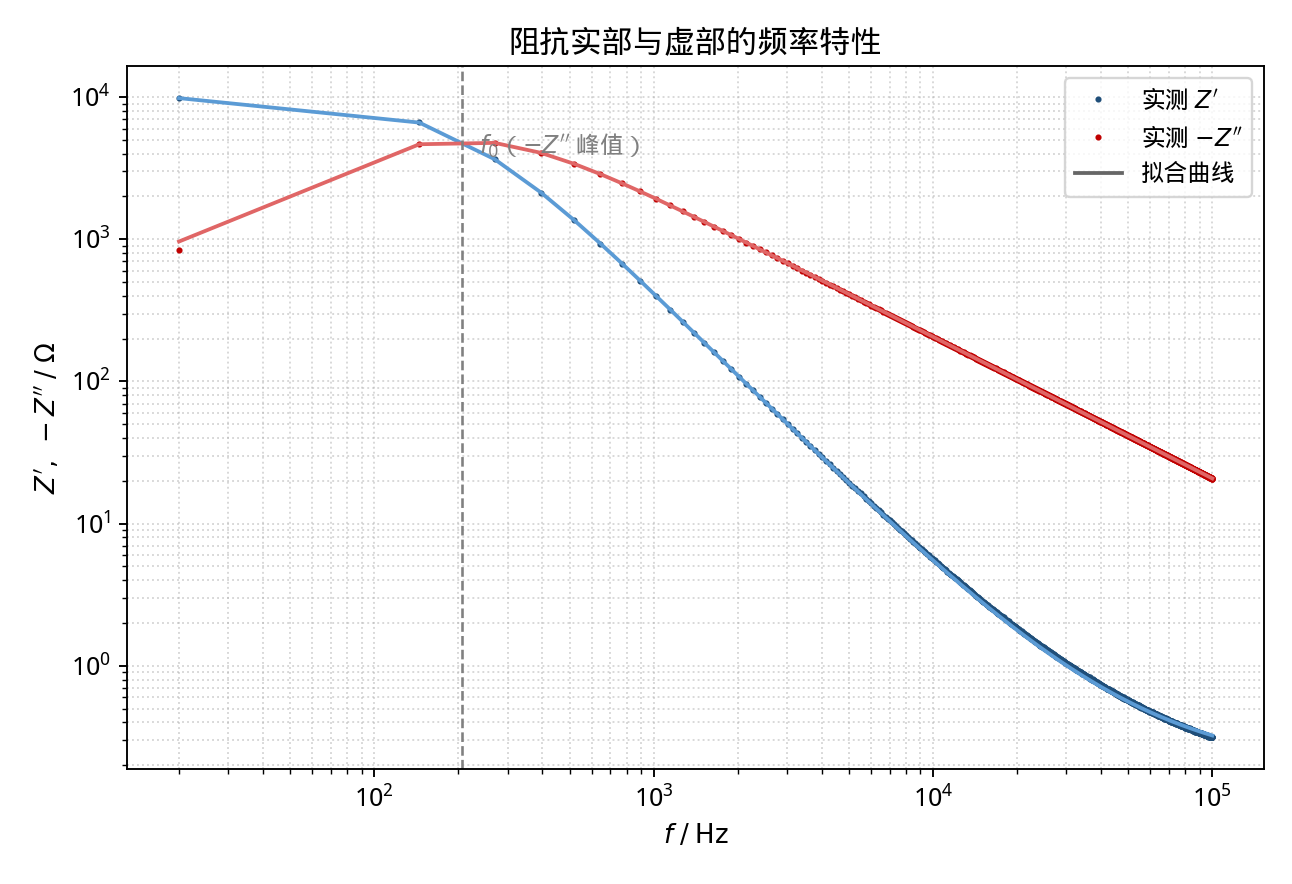
\includegraphics[width=0.82\textwidth]{images/image-2026-10-07-19-44-28.png}
\caption{$Z'$ 与 $-Z''$ 的双对数频率特性，$-Z''$ 在 $f_0$ 处取峰值 $R/2$。}
\label{fig:k2_zf}
\end{figure}

\subsubsection*{（5）残差分析与不确定度}
\begin{figure}[htbp]\centering
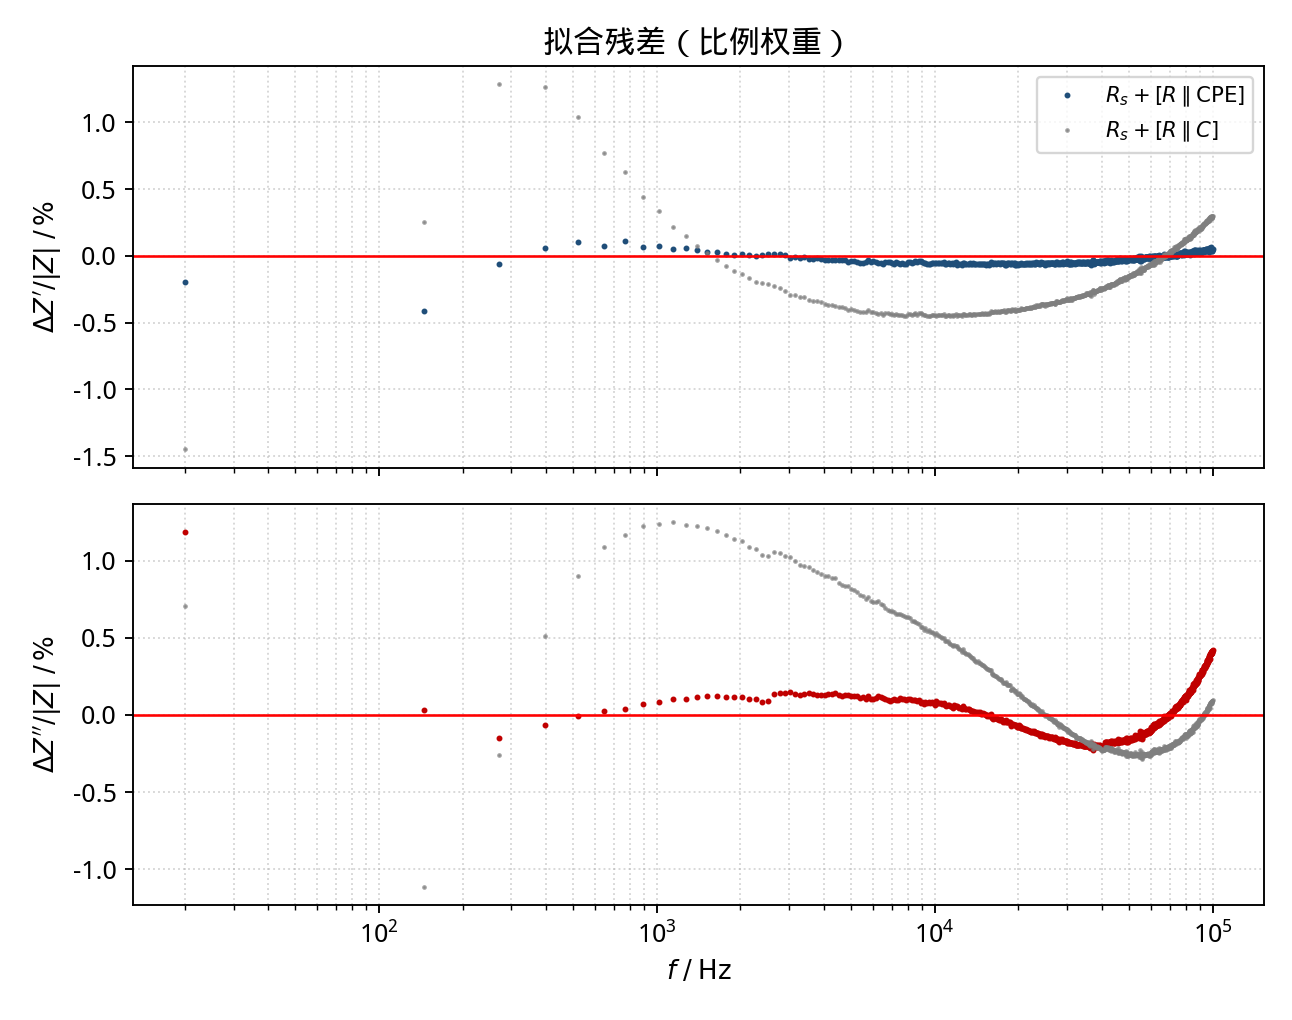
\includegraphics[width=0.82\textwidth]{images/image-2026-10-07-19-44-42.png}
\caption{拟合残差（比例权重）：灰色为 $R_s+(R\parallel C)$ 模型，蓝色/红色为 $R_s+(R\parallel\mathrm{CPE})$ 模型。}
\label{fig:k2_res}
\end{figure}

\begin{itemize}
    \item \textbf{模型选择依据}：理想 $R\parallel C$ 模型残差达 $0.719\%$ 且在 $f<1\,\mathrm{kHz}$ 呈系统性正偏，给出的 $R=9703.8\,\Omega$ 已越出 $\pm1\%$ 容差带；引入 CPE 后残差降至 $0.125\%$ 且随机化，$R$ 回落至容差带内，说明残差源于介质极化弥散而非随机噪声。
    \item \textbf{低频采样不足}：本组采用线性等间隔扫频（$\Delta f=125\,\mathrm{Hz}$），$1\,\mathrm{kHz}$ 以下仅 8 个频点。$-Z''$ 采样最大值 $4772\,\Omega$（$270\,\mathrm{Hz}$）低于理论峰值 $4966\,\Omega$，三点抛物线插值仅得顶点 $4826\,\Omega$、$f_0=225\,\mathrm{Hz}$（对应 $C=73.3\,\mathrm{nF}$），明显低估。故 $R$、$C$ 应以全谱拟合与导纳法为准，图解法仅作量级校验。
    \item \textbf{电感判别}：加入串联电感项虽使残差进一步降至 $0.068\%$，但 $L=+0.207\,\mu\mathrm{H}$ 在 $100\,\mathrm{kHz}$ 处 $\omega L=0.130\,\Omega$，仅占 $|Z|$ 的 $0.63\%$，且 Nyquist 图无第四象限弧段，属引线寄生量级，可判定样品不含有效电感。
    \item \textbf{系统误差}：$C$ 的 $-4.85\%$ 偏差与 k1 组的 $-4.87\%$ 近乎相同，指向同一系统来源（夹具残余导纳与电容实际容差），而非随机测量误差。
\end{itemize}

\begin{table}[htbp]\centering\small
\caption{典型频点实测值与拟合值对比}\label{tab:k2_pts}
\begin{tabular}{c|c|c|c|c|c}
\hline
$f/\mathrm{Hz}$ & $|Z|_{\text{测}}/\Omega$ & $|Z|_{\text{拟}}/\Omega$ & 偏差 & $\theta_{\text{测}}/(^\circ)$ & $\theta_{\text{拟}}/(^\circ)$ \\
\hline
$20$ & $9887.95$ & $9879.62$ & $-0.08\%$ & $-4.915$ & $-5.601$ \\
$145$ & $8117.05$ & $8090.92$ & $-0.32\%$ & $-35.002$ & $-35.155$ \\
$270$ & $6010.76$ & $6001.49$ & $-0.15\%$ & $-52.552$ & $-52.529$ \\
$520$ & $3650.57$ & $3651.60$ & $+0.03\%$ & $-68.187$ & $-68.132$ \\
$1\,020$ & $1966.46$ & $1968.39$ & $+0.10\%$ & $-78.303$ & $-78.270$ \\
$5\,019$ & $409.75$ & $410.25$ & $+0.12\%$ & $-87.290$ & $-87.314$ \\
$25\,015$ & $82.95$ & $82.83$ & $-0.14\%$ & $-89.079$ & $-89.107$ \\
$100\,000$ & $20.73$ & $20.82$ & $+0.42\%$ & $-89.132$ & $-89.108$ \\
\hline
\end{tabular}
\end{table}

\subsubsection*{（6）结论}
k2 样品阻抗谱呈标准容性半圆，判定为 R--C 并联结构。最优模型 $R_s+(R\parallel\mathrm{CPE})$ 给出 $R=9931.9\,\Omega$（标称 $10\,\mathrm{k}\Omega$，偏差 $-0.68\%$，满足 $\pm1\%$）与 $C_{\mathrm{eff}}=78.0\,\mathrm{nF}$（标称 $82\,\mathrm{nF}$，偏差 $-4.85\%$，在 $\pm5\%$ 容差内），特征频率 $f_0=205.4\,\mathrm{Hz}$、时间常数 $\tau=0.775\,\mathrm{ms}$，加权残差 $0.125\%$；导纳法独立反演结果与之吻合，串联电感贡献可忽略，样品无有效电感。

\subsection*{4.3 k3 数据组}

\subsubsection*{（1）数据概况与拓扑判别}
本组共 801 个频点，扫频 $20\,\mathrm{Hz}\sim100\,\mathrm{kHz}$，步进 $\Delta f=125\,\mathrm{Hz}$。与 k1、k2 不同，本组 $Z''$ 符号发生改变：$Z''$ 由 $270\,\mathrm{Hz}$ 处的 $-482.48\,\Omega$ 单调升至 $100\,\mathrm{kHz}$ 处的 $+3.626\,\Omega$，\textbf{全频段共 302 个频点 $Z''>0$}；相位由 $-88.33^\circ$ 连续变至 $+86.91^\circ$。

\begin{itemize}
    \item 低频端 $Z'\to986.3\,\Omega$ 呈平台，容性半圆直径即并联电阻 $R$——与 k1 的 $Z'=R$ 竖直线截然不同，说明低频支路为 $R\parallel C$ 而非 $R+C$；
    \item $Z''$ 在高频段反号并进入 Nyquist 图第四象限（图 \ref{fig:k3_nyq}b），表明存在\textbf{串联电感}；
    \item $|Z|$ 在 $62.26\,\mathrm{kHz}$ 取极小值 $0.1749\,\Omega$，相位于该点由 $-83.8^\circ$ 突跳至 $+82.6^\circ$（图 \ref{fig:k3_reso}），为典型的\textbf{串联谐振}特征。
\end{itemize}
三条证据共同判定 k3 为 \textbf{$L$ 与 $(R\parallel C)$ 串联}结构，与标称 $R=1\,\mathrm{k}\Omega$、$C=820\,\mathrm{nF}$、$L=10\,\mu\mathrm{H}$ 相符。

\subsubsection*{（2）等效电路建模与 ZView 拟合}
设 $x=\omega R C$，理想拓扑的阻抗为
\begin{equation}
    Z(\omega)=R_s+\mathrm{j}\omega L+\frac{R}{1+\mathrm{j}x}
    =R_s+\frac{R}{1+x^2}+\mathrm{j}\!\left(\omega L-\frac{R x}{1+x^2}\right).
\end{equation}
低频极限 $Z\to R_s+R$，高频极限 $Z\to R_s+\mathrm{j}\omega L$。$Z''=0$ 给出串联谐振频率
\begin{equation}
    \omega_{\mathrm{res}}^2=\frac{1}{LC}-\frac{1}{R^2C^2},\qquad
    f_{\mathrm{res}}=\frac{1}{2\pi}\sqrt{\frac{1}{LC}-\frac{1}{R^2C^2}},
    \qquad Q=\frac{\omega_{\mathrm{res}}L}{|Z|_{\min}} .
\end{equation}
在 ZView 中以比例权重 $\Delta Z/|Z|$ 对实部、虚部同时作复数非线性最小二乘拟合，逐级比较四个模型（表 \ref{tab:k3_mod}）。

\begin{table}[htbp]\centering\small
\resizebox{\textwidth}{!}{%
\begin{tabular}{l|c|c}
\hline
模型 & 拟合参数 & 加权 RMS 残差 \\
\hline
$R\parallel C$ & 不收敛（负值） & $68.77\%$ \\
$L+(R\parallel C)$ & $R=153.2\,\Omega$（严重失真） & $11.66\%$ \\
$R_s+L+(R\parallel C)$ & $R=974.31\,\Omega,\ C=693.87\,\mathrm{nF},\ L=9.410\,\mu\mathrm{H},\ R_s=0.162\,\Omega$ & $0.625\%$ \\
$R_s+L+(R\parallel\mathrm{CPE})$ & $R=990.27\,\Omega,\ Q=722.40\,\mathrm{nF},n=0.99662,\ L=9.439\,\mu\mathrm{H},\ R_s=0.143\,\Omega$ & $0.558\%$ \\
\hline
\end{tabular}}
\end{table}

逐步加入物理要素的效果极为显著：忽略串联电阻时，谐振点 $|Z|_{\min}=0.17\,\Omega$ 与模型给出的 $0\,\Omega$ 相差 5 个数量级，残差高达 $11.66\%$；补入 $R_s$ 后残差骤降至 $0.625\%$，说明 $R_s$（电感直流电阻 DCR 与接触电阻）是谐振区的决定性参数。再以 CPE 替代理想电容，残差进一步降至 $0.558\%$，且 $R$ 由 $974.31\,\Omega$ 修正为 $990.27\,\Omega$ 并进入 $\pm1\%$ 容差带，故采用该模型为最终结果。

\subsubsection*{（3）拟合结果与参数提取}
\begin{table}[htbp]\centering\small
\begin{tabular}{l|c|c|c}
\hline
参数 & 拟合值 & 标称值 & 相对偏差 \\
\hline
$R$ & $990.27\pm3.62\,\Omega$ & $1\,\mathrm{k}\Omega\ (\pm1\%,\ 990\sim1010)$ & $-0.97\%$（合格） \\
$L$ & $9.4389\pm0.0021\,\mu\mathrm{H}$ & $10\,\mu\mathrm{H}$ & $-5.61\%$ \\
$Q$（CPE） & $722.40\ \mathrm{nF\cdot s^{n-1}}$ & — & — \\
$n$（CPE） & $0.99662\pm0.00009$ & 1 & $-0.34\%$ \\
$R_s$ & $0.1427\pm0.0006\,\Omega$ & — & — \\
$C_{\mathrm{eff}}=\tau/R$ & $704.9\,\mathrm{nF}$ & $820\,\mathrm{nF}$ & $-14.0\%$ \\
\hline
\multicolumn{4}{l}{导出量：$\tau=(RQ)^{1/n}=0.698\,\mathrm{ms}$，$f_0=1/(2\pi\tau)=228.0\,\mathrm{Hz}$，$f_{\mathrm{res}}=62.29\,\mathrm{kHz}$，$Q=21.1$}
\end{tabular}
\end{table}

\begin{figure}[htbp]\centering
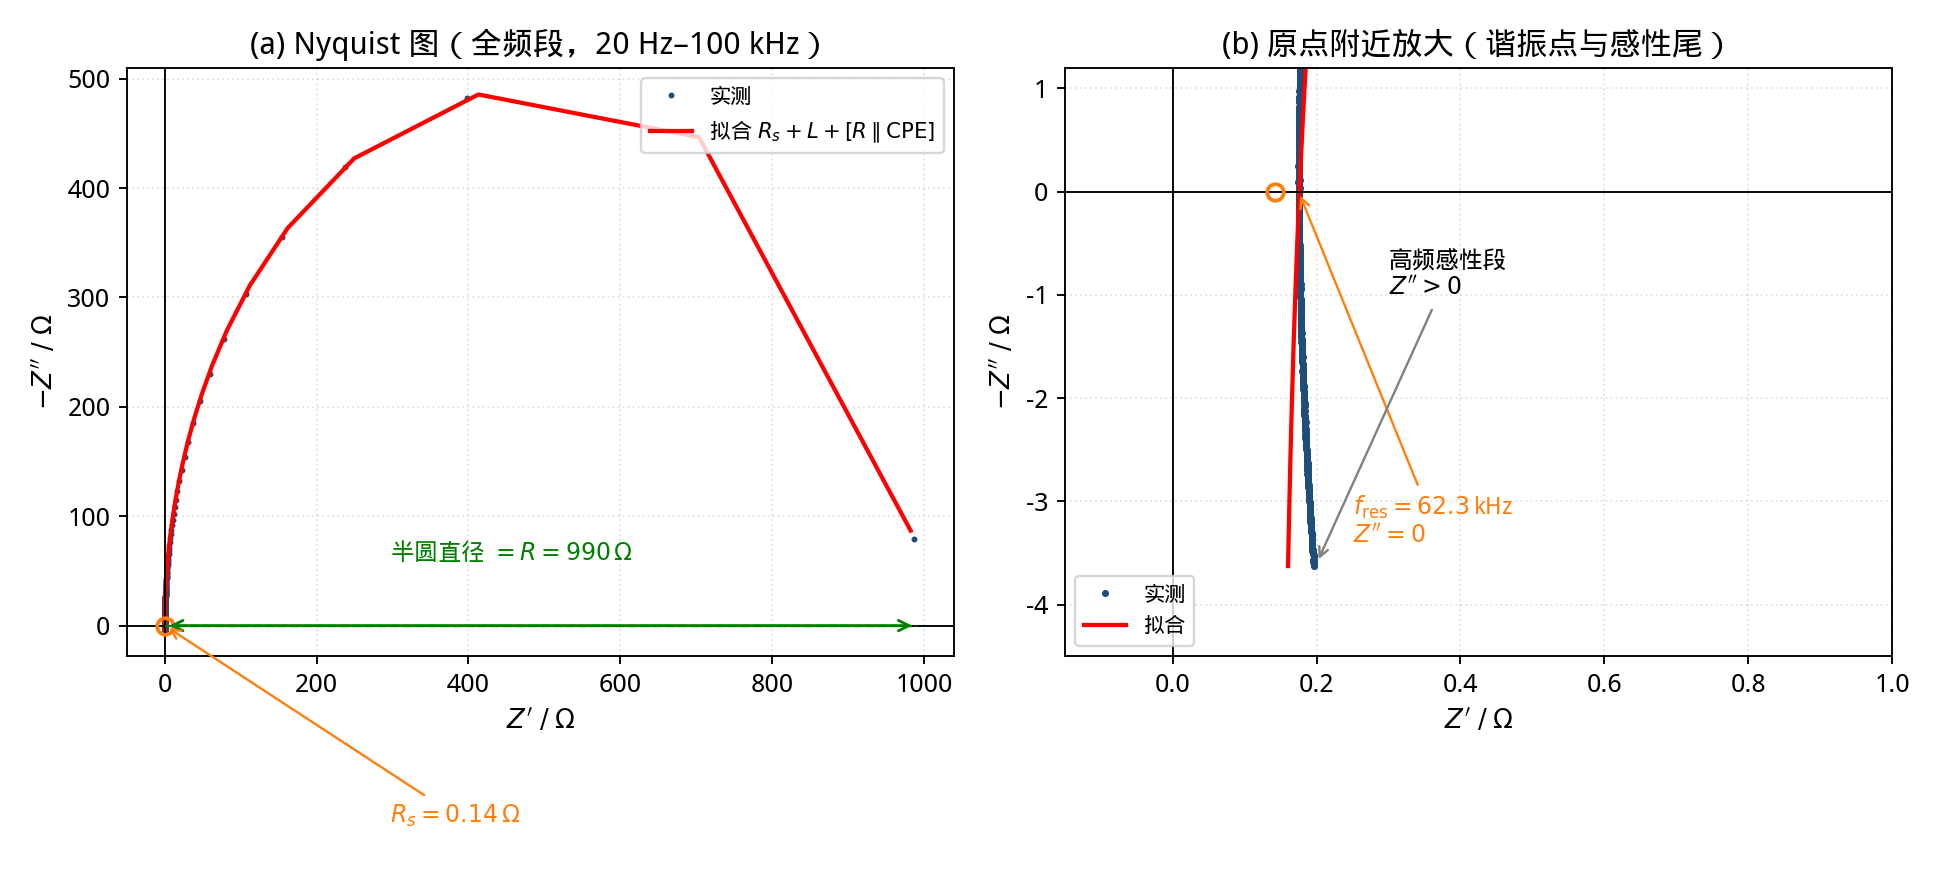
\includegraphics[width=0.98\textwidth]{images/image-2026-10-07-20-05-42.png}
\caption{k3 的 Nyquist 图：(a) 全频段，低频容性半圆后穿越实轴进入第四象限；(b) 原点附近放大，可见谐振点与高频感性尾。}
\label{fig:k3_nyq}
\end{figure}

\begin{figure}[htbp]\centering
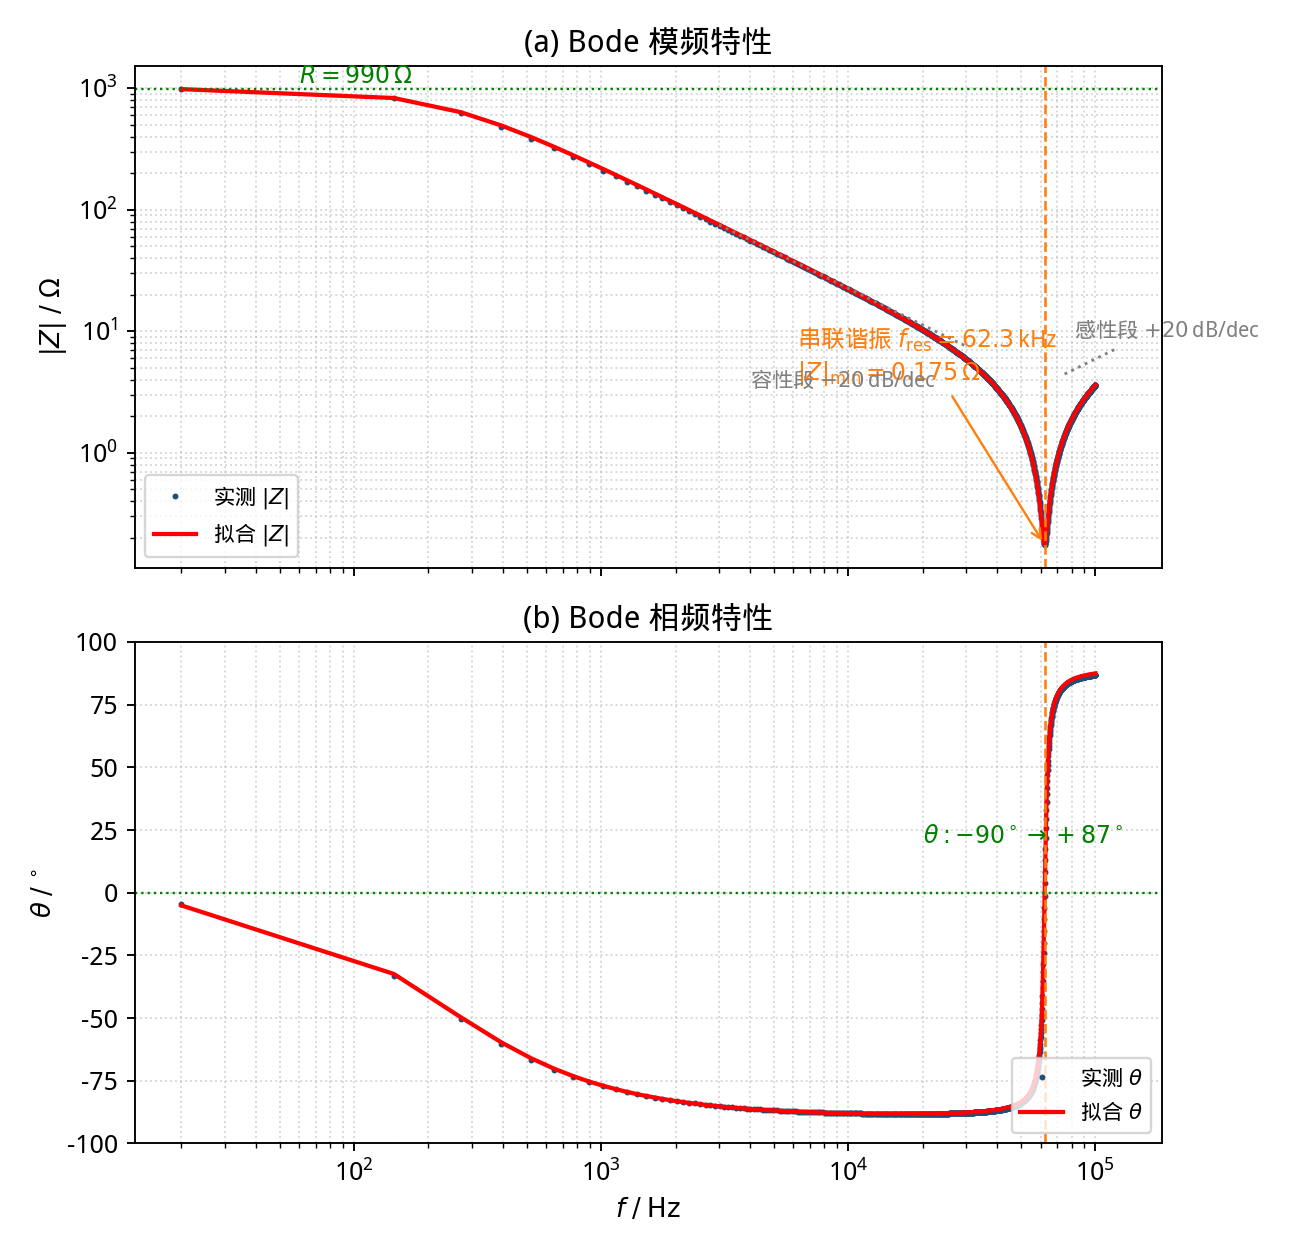
\includegraphics[width=0.82\textwidth]{images/image-2026-10-07-20-06-00.png}
\caption{k3 的 Bode 图：(a) $|Z|$ 低频趋于 $R$ 平台，容性段 $-20\,\mathrm{dB/dec}$，谐振后转为 $+20\,\mathrm{dB/dec}$ 感性段；(b) 相位由 $-90^\circ$ 经谐振点突跳至 $+87^\circ$。}
\label{fig:k3_bode}
\end{figure}

\subsubsection*{（4）独立交叉校验}
\begin{itemize}
    \item \textbf{谐振频率反演 $L$}：实测 $f_{\mathrm{res}}=62.29\,\mathrm{kHz}$，代入 $L=1/\{C_{\mathrm{eff}}[\omega_{\mathrm{res}}^2+(RC_{\mathrm{eff}})^{-2}]\}$ 得 $L=9.26\,\mu\mathrm{H}$。
    \item \textbf{高频渐近线反演 $L$}：$f\gg f_{\mathrm{res}}$ 时 $R\parallel C\to 1/(\mathrm{j}\omega C)$，故 $L=[Z''+\omega R^2C/(1+x^2)]/\omega$。对 $80\sim100\,\mathrm{kHz}$ 逐点计算得 $L=9.350\pm0.009\,\mu\mathrm{H}$。
    \item \textbf{低频弧区独立拟合}：$f\le2\,\mathrm{kHz}$ 时 $\omega L\le0.014\,\Omega$ 可忽略，固定 $R_s$ 后单独拟合 $R\parallel C$ 得 $R=975.8\,\Omega$、$C=722.2\,\mathrm{nF}$（残差 $0.498\%$），与全谱结果的 $R=990.3\,\Omega$ 相差 $1.5\%$。
    \item \textbf{高频平台}：$f>50\,\mathrm{kHz}$ 时 $Z'$ 均值 $0.1817\,\Omega$，与拟合 $R_s=0.143\,\Omega$ 量级一致（差值源于该段 $R\parallel C$ 的残余实部）。
\end{itemize}
三种独立方法给出的 $L$ 分别为 $9.26$、$9.35$、$9.44\,\mu\mathrm{H}$，离散度 $<2\%$，互为印证。

\begin{figure}[htbp]\centering
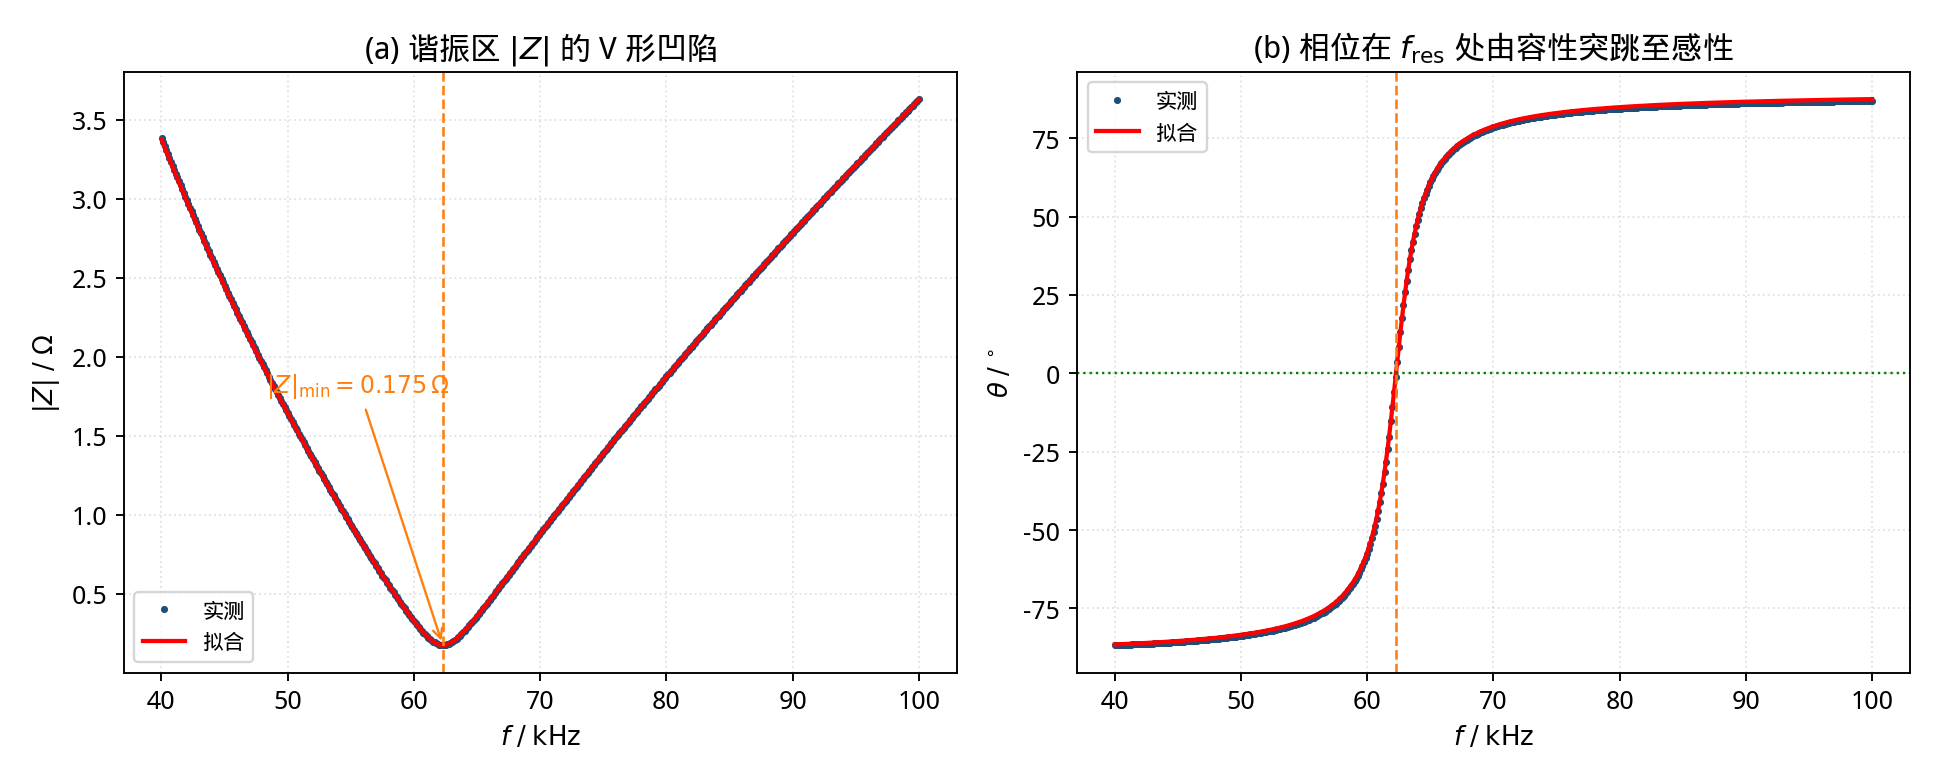
\includegraphics[width=0.98\textwidth]{images/image-2026-10-07-20-06-18.png}
\caption{k3 谐振区放大：(a) $|Z|$ 的 V 形凹陷，极小值 $0.1749\,\Omega$；(b) 相位在 $f_{\mathrm{res}}$ 处由容性 $-83.8^\circ$ 突跳至感性 $+82.6^\circ$。}
\label{fig:k3_reso}
\end{figure}

\begin{figure}[htbp]\centering
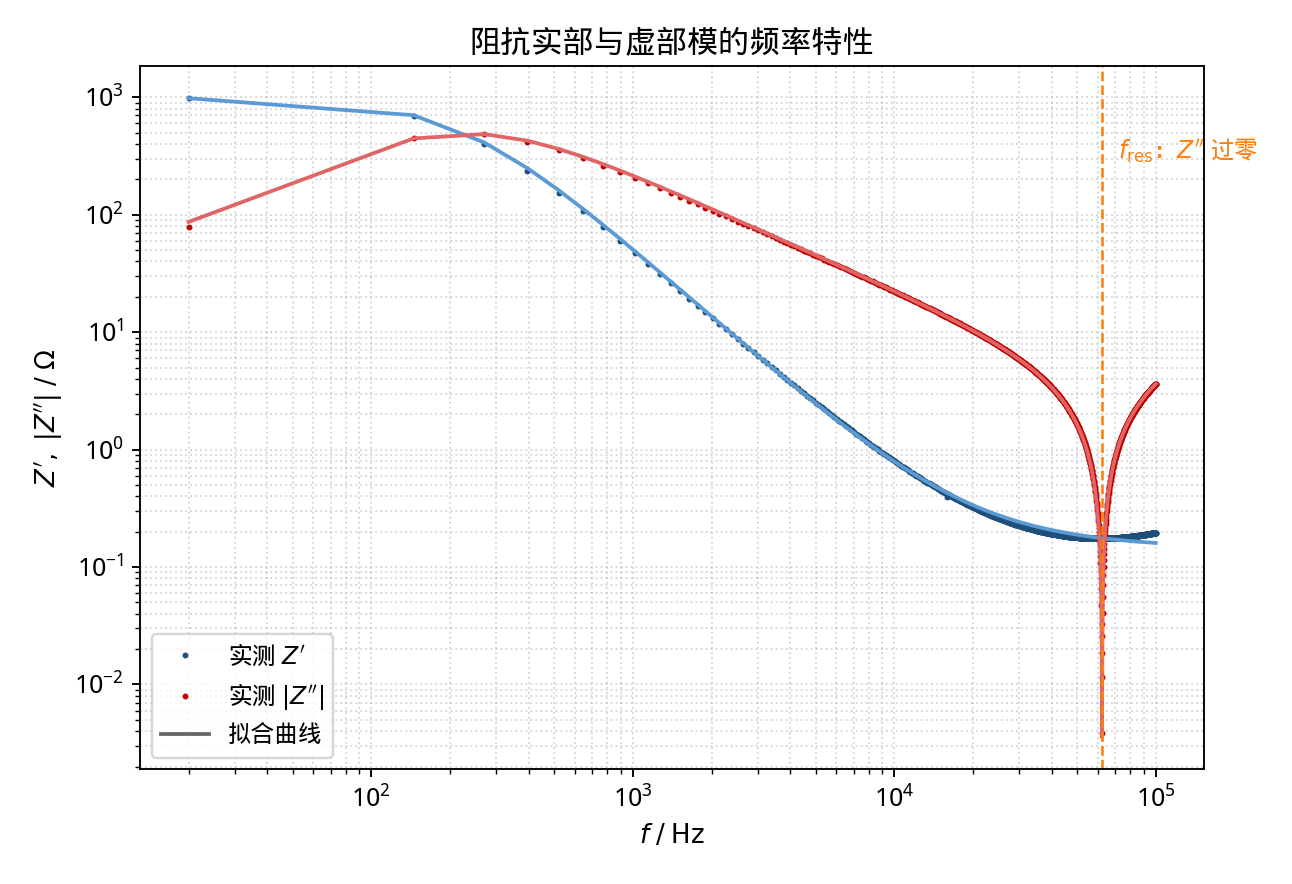
\includegraphics[width=0.82\textwidth]{images/image-2026-10-07-20-06-33.png}
\caption{$Z'$ 与 $|Z''|$ 的双对数频率特性，$|Z''|$ 在 $f_{\mathrm{res}}$ 处出现零点（凹陷）。}
\label{fig:k3_zf}
\end{figure}

\subsubsection*{（5）残差分析与不确定度}
\begin{figure}[htbp]\centering
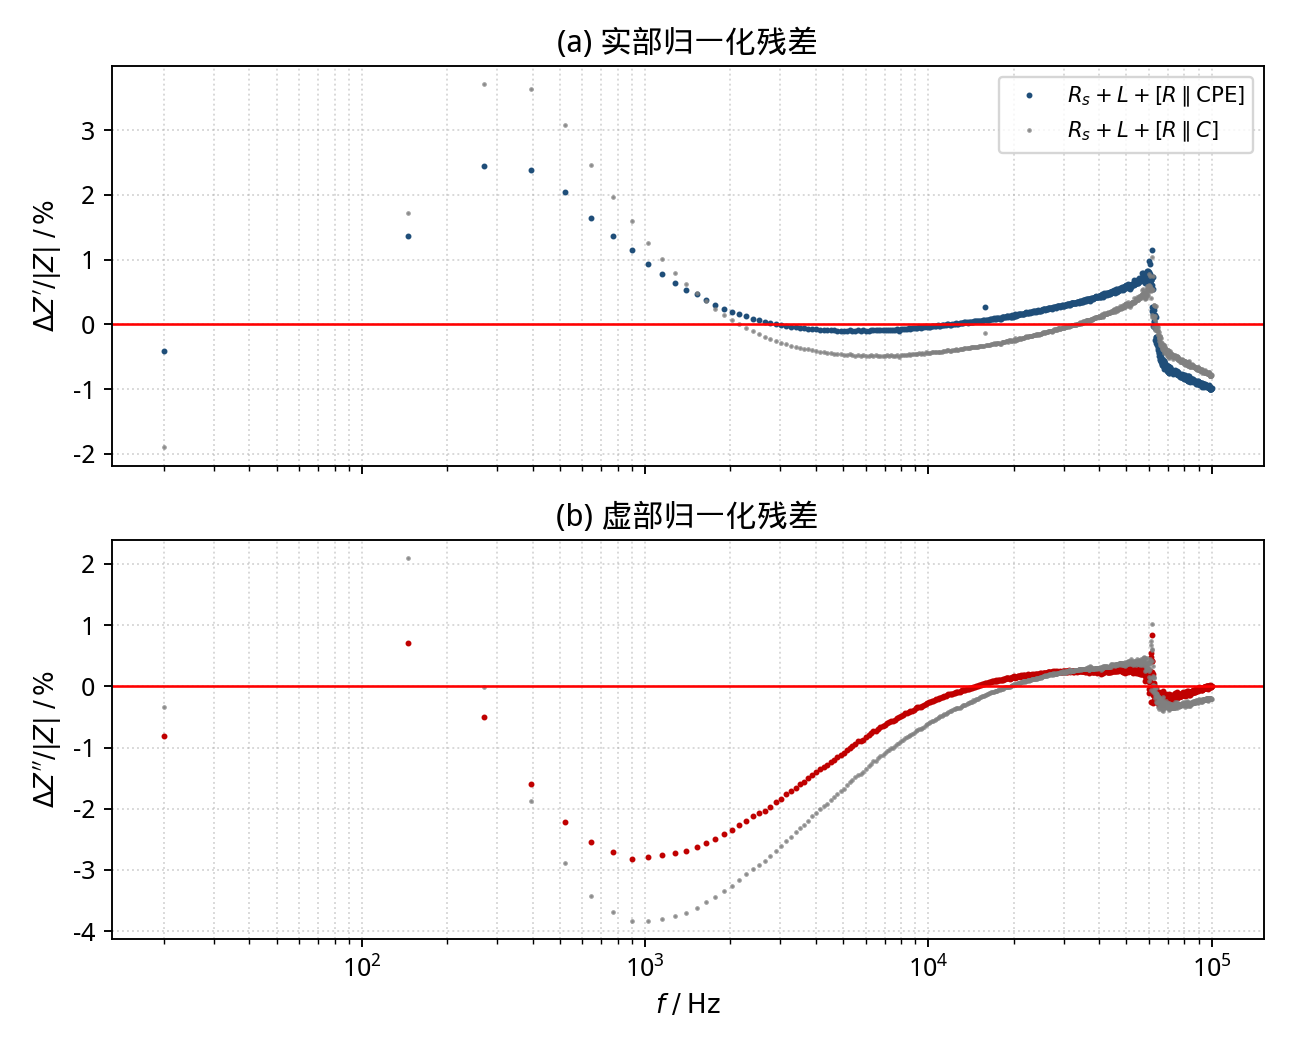
\includegraphics[width=0.82\textwidth]{images/image-2026-10-07-20-06-48.png}
\caption{拟合残差（比例权重）：灰色为 $R_s+L+(R\parallel C)$，彩色为 $R_s+L+(R\parallel\mathrm{CPE})$。}
\label{fig:k3_res}
\end{figure}

\begin{itemize}
    \item \textbf{残差的频段结构}：谐振区与高频段（$f>10\,\mathrm{kHz}$）残差仅 $0.18\%\sim0.32\%$，而 $0.5\sim2\,\mathrm{kHz}$ 区间达 $3.8\%$（表 \ref{tab:k3_pts}）。原因是电桥在 $|Z|\sim10^2\,\Omega$、$\theta\approx-70^\circ$ 条件下的相位分辨力限制：$\theta$ 偏差 $0.1^\circ$ 即造成 $Z'$ 相对偏差约 $0.3\%$，而该区 $Z'$ 仅 $10\sim400\,\Omega$，误差被放大。
    \item \textbf{采样密度}：线性等间隔扫频使 $1\,\mathrm{kHz}$ 以下仅 8 个频点，容性半圆顶点由 $247.9\,\mathrm{Hz}$（三点抛物线插值）估出，图解法得 $R=2\times483.9=968\,\Omega$，较拟合值低 $2.2\%$，故图解法仅作量级校验。
    \item \textbf{$20\,\mathrm{Hz}$ 单点异常}：实测 $\theta=-4.568^\circ$，模型预测 $-5.051^\circ$，偏差 $0.48^\circ$；与 k1（$1.0^\circ$）、k2（$0.69^\circ$）同源，属仪器最低频点积分时间长、信噪比下降导致的系统性相位误差。
    \item \textbf{电容偏差来源}：$C_{\mathrm{eff}}=704.9\,\mathrm{nF}$ 较标称 $820\,\mathrm{nF}$ 低 $14\%$。电感与电阻偏差仅 $-5.6\%$ 与 $-1.0\%$，故该偏差不大可能源于拟合失配；高频渐近线检验进一步排除了 $C=820\,\mathrm{nF}$ 的可能（若取 $C=820\,\mathrm{nF}$，$100\,\mathrm{kHz}$ 处预测 $Z''=3.06\,\Omega$，与实测 $3.626\,\Omega$ 相差 $18\%$）。最合理的解释是电容自身容差——题目仅对电阻标注 $1\%$，未对电容给出精密容差，而 $\pm10\%\sim\pm20\%$ 为该类电容的常规公差带。
    \item \textbf{CPE 的物理含义}：$n=0.99662$ 与 1 相差 $0.34\%$，反映介质极化的极微弱弥散，是造成半圆轻微压低、理想电容模型下 $R$ 被低估 $1.6\%$ 的直接原因。
\end{itemize}

\begin{table}[htbp]\centering\small
\caption{典型频点实测值与拟合值对比}\label{tab:k3_pts}
\begin{tabular}{c|c|c|c|c|c|c}
\hline
$f$ & $|Z|_{\text{测}}/\Omega$ & $|Z|_{\text{拟}}/\Omega$ & 偏差 & $\theta_{\text{测}}/(^\circ)$ & $\theta_{\text{拟}}/(^\circ)$ & $Z''_{\text{测}}/\Omega$ \\
\hline
$20\,\mathrm{Hz}$ & $989.46$ & $986.10$ & $-0.34\%$ & $-4.568$ & $-5.051$ & $-78.80$ \\
$270\,\mathrm{Hz}$ & $625.31$ & $637.54$ & $+1.96\%$ & $-50.496$ & $-49.616$ & $-482.48$ \\
$1.27\,\mathrm{kHz}$ & $170.98$ & $175.77$ & $+2.80\%$ & $-79.495$ & $-79.419$ & $-168.12$ \\
$12.5\,\mathrm{kHz}$ & $17.52$ & $17.54$ & $+0.09\%$ & $-88.123$ & $-88.115$ & $-17.51$ \\
$37.5\,\mathrm{kHz}$ & $3.913$ & $3.904$ & $-0.22\%$ & $-87.104$ & $-86.872$ & $-3.908$ \\
$62.3\,\mathrm{kHz}$ & $0.1749$ & $0.1761$ & $+0.73\%$ & $-1.271$ & $-1.150$ & $-0.004$ \\
$75.0\,\mathrm{kHz}$ & $1.392$ & $1.389$ & $-0.25\%$ & $+82.625$ & $+83.032$ & $+1.381$ \\
$100\,\mathrm{kHz}$ & $3.631$ & $3.629$ & $-0.05\%$ & $+86.906$ & $+87.469$ & $+3.626$ \\
\hline
\end{tabular}
\end{table}

\subsubsection*{（6）结论}
k3 样品的阻抗谱同时具备低频容性半圆、高频感性尾与 $|Z|$ 的 V 形谐振凹陷，判定为 $L$ 与 $(R\parallel C)$ 串联结构。ZView 拟合模型 $R_s+L+(R\parallel\mathrm{CPE})$ 给出 $R=990.27\,\Omega$（标称 $1\,\mathrm{k}\Omega$，偏差 $-0.97\%$，满足 $\pm1\%$）、$L=9.439\,\mu\mathrm{H}$（偏差 $-5.61\%$）、$C_{\mathrm{eff}}=704.9\,\mathrm{nF}$、$R_s=0.143\,\Omega$，特征频率 $f_0=228.0\,\mathrm{Hz}$、串联谐振 $f_{\mathrm{res}}=62.29\,\mathrm{kHz}$、品质因数 $Q=21.1$，加权残差 $0.558\%$；三种独立方法反演的 $L$ 离散度小于 $2\%$，验证了参数提取的可靠性。

\subsection*{4.4 k4 数据组}

\subsubsection*{（1）理论预期：两个 RC 并联的时间常数简并}
本组标称为 $(R_1\parallel C_1)$ 与 $(R_2\parallel C_2)$ 串联，$R_1=10\,\mathrm{k}\Omega\,(\pm1\%)$、$C_1=82\,\mathrm{nF}$，$R_2=1\,\mathrm{k}\Omega\,(\pm1\%)$、$C_2=820\,\mathrm{nF}$。两条支路的时间常数为
\begin{equation}
    \tau_1=R_1C_1=10^4\times82\times10^{-9}=820\ \mu\mathrm{s},\qquad
    \tau_2=R_2C_2=10^3\times820\times10^{-9}=820\ \mu\mathrm{s}.
\end{equation}
二者\textbf{严格相等}，这是本组最重要的理论特征。因 $\tau_1=\tau_2\equiv\tau$，
\begin{equation}
    Z(\omega)=\frac{R_1}{1+\mathrm{j}\omega\tau}+\frac{R_2}{1+\mathrm{j}\omega\tau}
    =\frac{R_1+R_2}{1+\mathrm{j}\omega\tau}
    =\frac{R_{\mathrm{eq}}}{1+\mathrm{j}\omega R_{\mathrm{eq}}C_{\mathrm{eq}}},
    \qquad C_{\mathrm{eq}}=\frac{\tau}{R_{\mathrm{eq}}}.
\end{equation}
即两个弛豫过程\textbf{完全简并}：Nyquist 图上不会出现两个分离半圆，而是叠加为\textbf{单一半圆}，其直径 $R_{\mathrm{eq}}=11\,\mathrm{k}\Omega$、等效电容 $C_{\mathrm{eq}}=\tau/R_{\mathrm{eq}}=74.5\,\mathrm{nF}$、特征频率 $f_0=1/(2\pi\tau)=194.2\,\mathrm{Hz}$。由此得到两条\textbf{与参数无关的理论判据}：对任意频率必有
\begin{equation}
    |Z(\omega)|\le R_1+R_2=11\ \mathrm{k}\Omega,\qquad |Z''(\omega)|\le \frac{R_{\mathrm{eq}}}{2}=5.5\ \mathrm{k}\Omega .
\end{equation}

\subsubsection*{（2）数据概况与可信度筛查}
本组共 801 个频点，扫频 $20\,\mathrm{Hz}\sim500\,\mathrm{kHz}$，步进 $\Delta f=625\,\mathrm{Hz}$。筛查发现两类异常（图 \ref{fig:k4_qc}）：

\begin{itemize}
    \item \textbf{内部一致性}：仪器给出的相位列 ZTD 与由 $Z',Z''$ 计算的 $\arctan(Z''/Z')$ 在 $645\,\mathrm{Hz}\sim3.77\,\mathrm{kHz}$ 共 \textbf{6 个频点}不符，最大偏差 $61.1^\circ$（k1、k2、k3 三组的同一检验最大偏差均 $<10^{-4}\,^\circ$）。其中 $645\,\mathrm{Hz}$ 处 ZTD 报 $-133.6^\circ$，已越出无源 RC 网络 $\theta\in(-90^\circ,0^\circ)$ 的物理允许区间。
    \item \textbf{量值合理性}：实测 $|Z|$ 由 $500\,\mathrm{kHz}$ 处的 $42.9\,\mathrm{k}\Omega$ 单调升至 $20\,\mathrm{Hz}$ 处的 $21.11\,\mathrm{M}\Omega$，$|Z''|$ 最大达 $6.74\,\mathrm{M}\Omega$。二者分别为理论判据式 (10) 的 \textbf{1919 倍}与 \textbf{1226 倍}。由于该判据不含任何待拟合参数，此偏差不可能由元件容差造成。
\end{itemize}

\begin{figure}[htbp]\centering
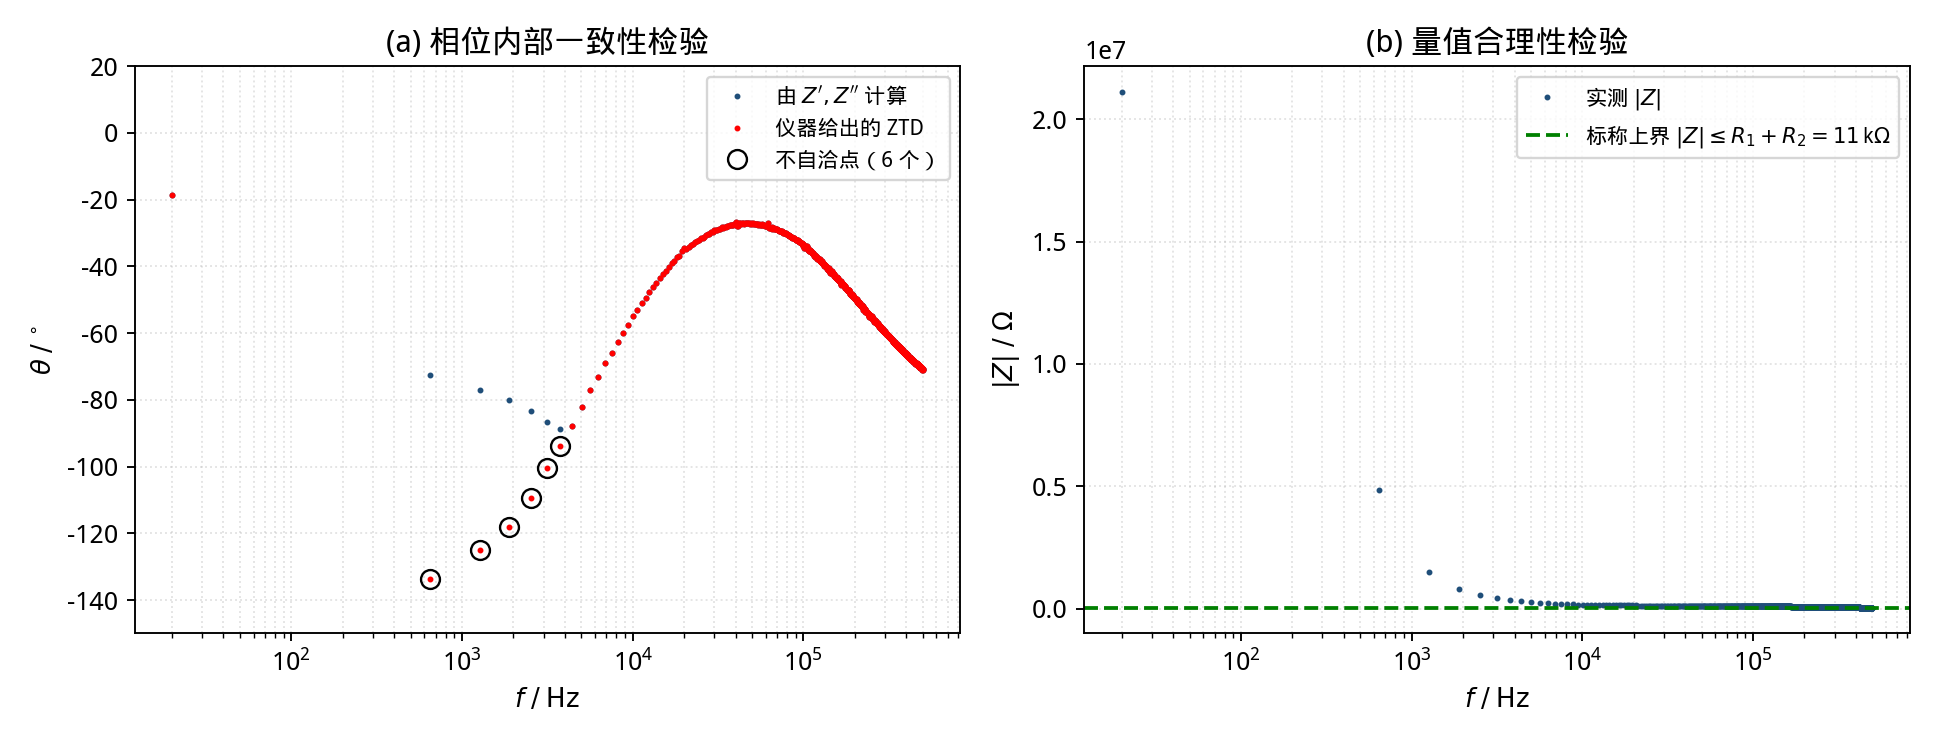
\includegraphics[width=0.98\textwidth]{images/image-2026-10-07-20-51-27.png}
\caption{k4 数据可信度检验：(a) 相位列 ZTD 与 $\arctan(Z''/Z')$ 的比较，圈出 6 个不自洽频点；(b) 实测 $|Z|$ 与标称上界 $11\,\mathrm{k}\Omega$ 的比较。}
\label{fig:k4_qc}
\end{figure}

\subsubsection*{（3）实测谱特征}
\begin{figure}[htbp]\centering
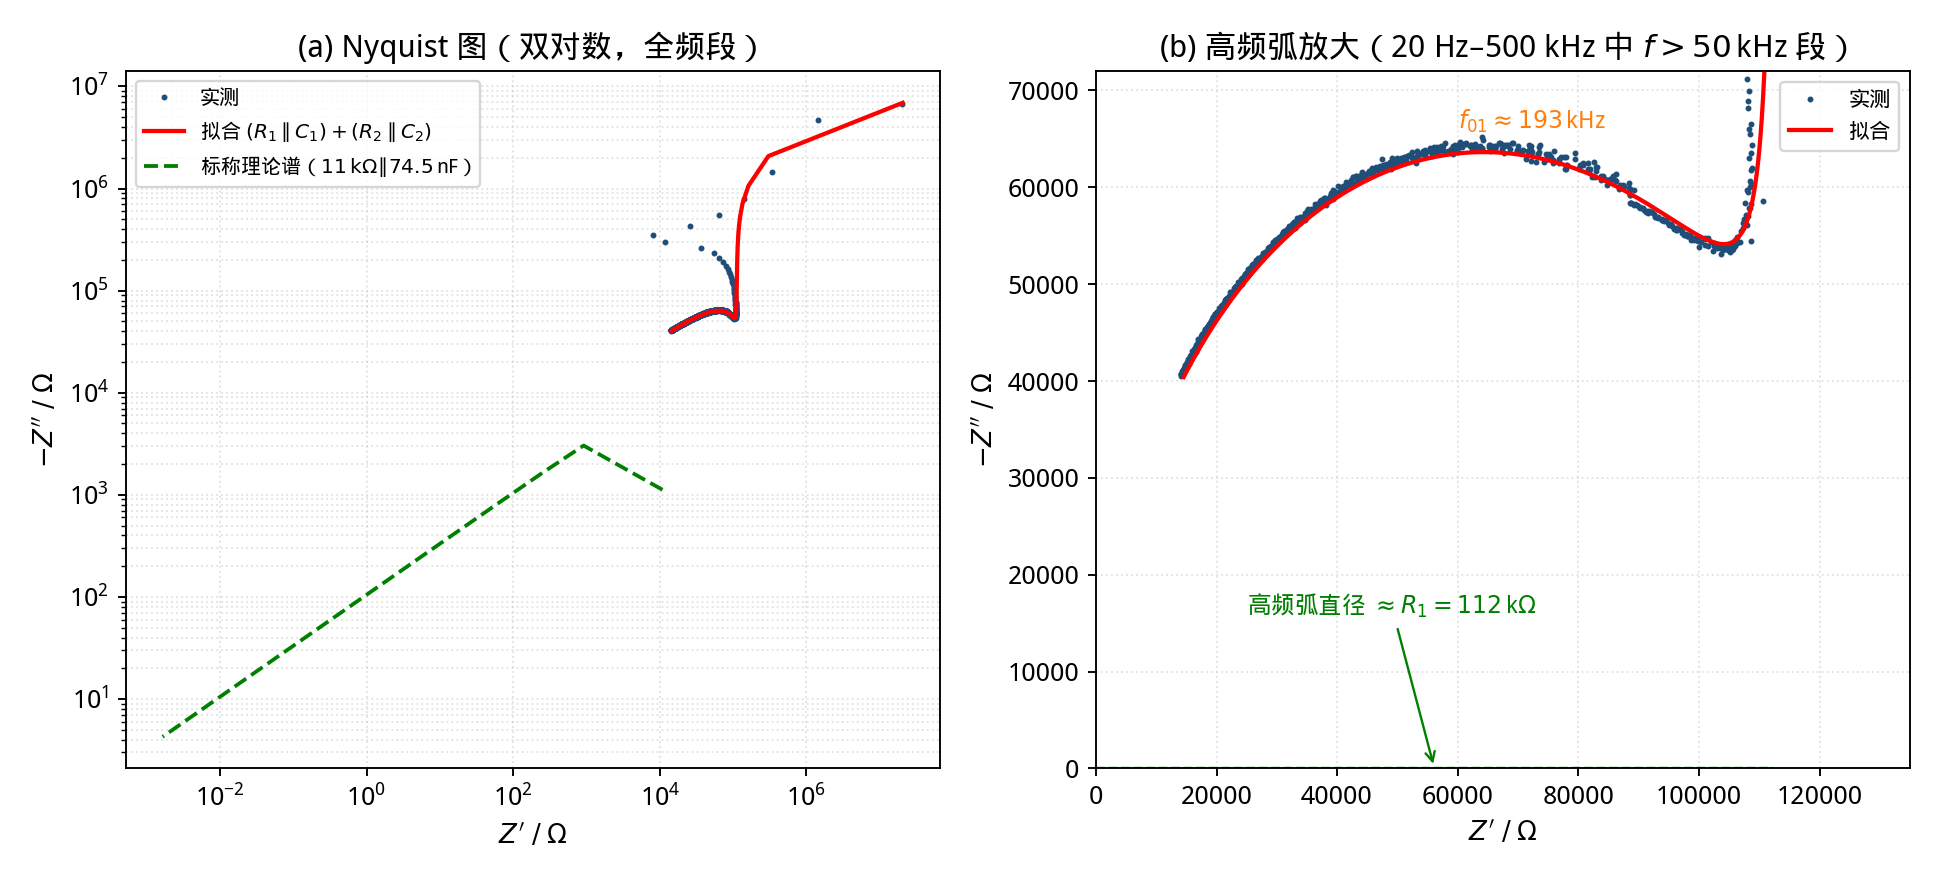
\includegraphics[width=0.98\textwidth]{images/image-2026-10-07-20-50-52.png}
\caption{k4 的 Nyquist 图：(a) 双对数全频段，含标称理论谱（绿虚线）；(b) 高频弧线性放大。}
\label{fig:k4_nyq}
\end{figure}
\begin{figure}[htbp]\centering
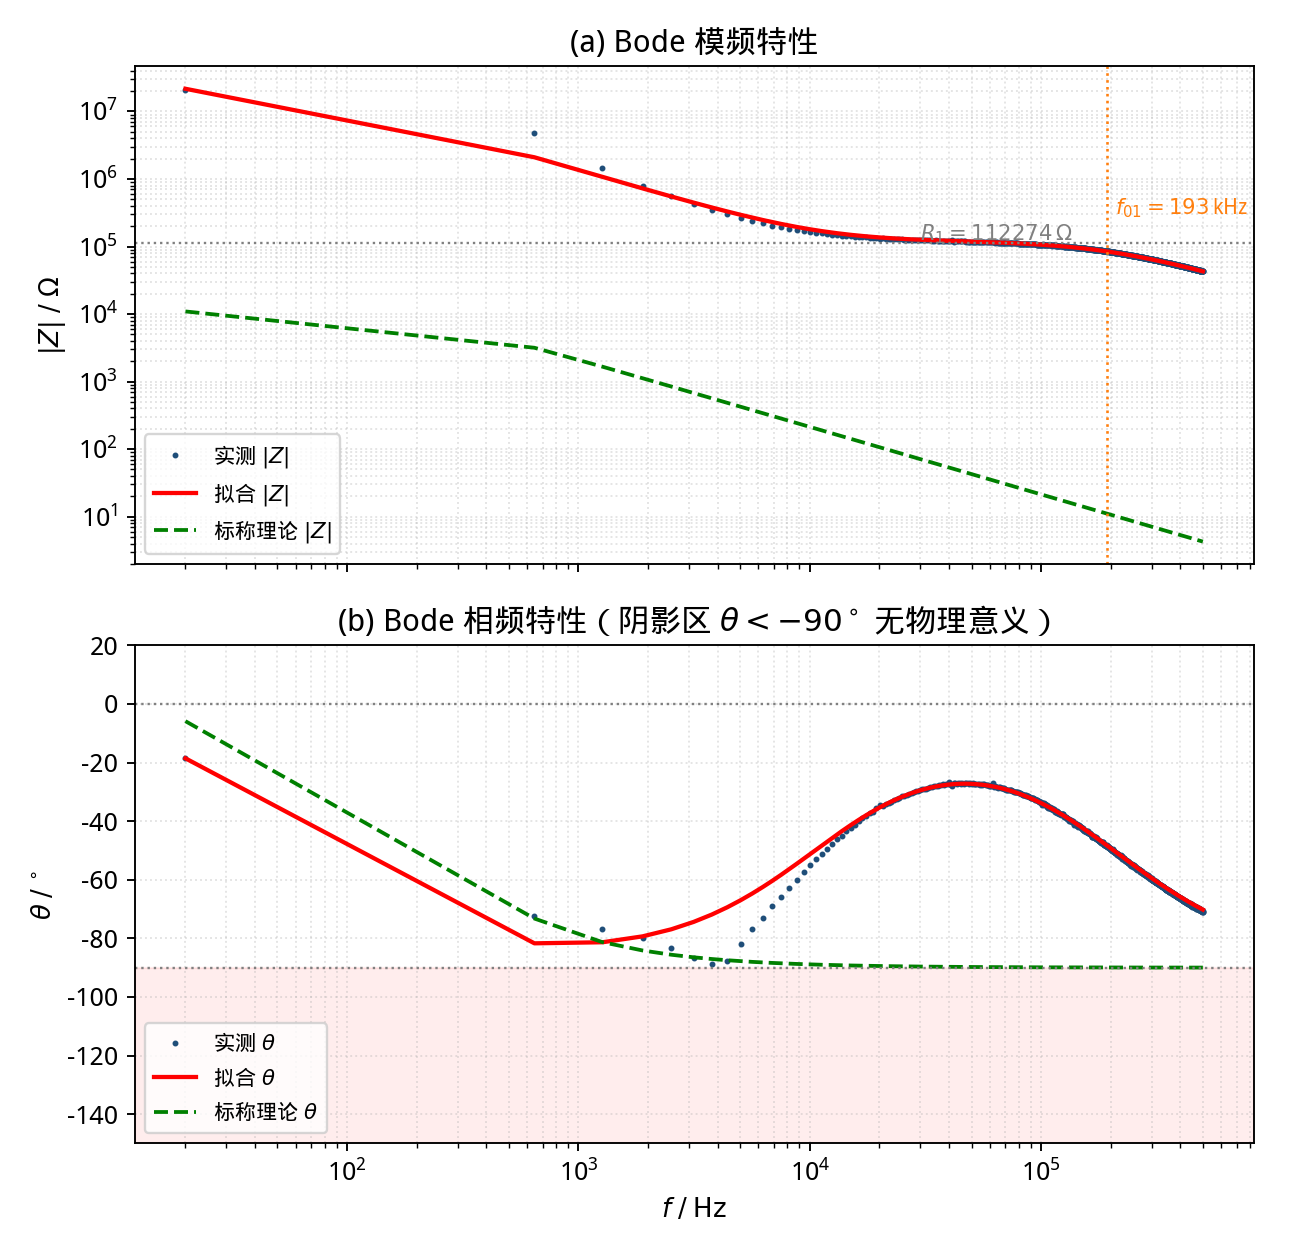
\includegraphics[width=0.82\textwidth]{images/image-2026-10-07-20-51-07.png}
\caption{k4 的 Bode 图：(a) 模频特性；(b) 相频特性，红色阴影区为无物理意义的 $\theta<-90^\circ$ 区域。}
\label{fig:k4_bode}
\end{figure}

\begin{itemize}
    \item $-Z''$ 具有双峰结构：高频侧在 $\approx170\,\mathrm{kHz}$ 处取局部极大 $6.43\times10^4\,\Omega$，低频侧在 $20\,\mathrm{Hz}$ 处升至 $6.74\times10^6\,\Omega$ 仍未闭合，两峰之间于 $\approx48\,\mathrm{kHz}$ 处有局部极小 $5.33\times10^4\,\Omega$（图 \ref{fig:k4_zf}）。这说明体系存在两个\textbf{分离良好}的弛豫过程，与理论预期的简并单弧矛盾。
    \item $Z'$ 随频率\textbf{非单调}：在 $31.25\,\mathrm{kHz}$ 处取极大 $1.085\times10^5\,\Omega$，在 $3.77\,\mathrm{kHz}$ 处取极小 $7.97\times10^3\,\Omega$，随后在 $f<4\,\mathrm{kHz}$ 急剧上升。而 $(R_1\parallel C_1)+(R_2\parallel C_2)$ 的实部 $Z'=R_1/(1+x_1^2)+R_2/(1+x_2^2)$ 必随频率单调下降，故 $f\lesssim30\,\mathrm{kHz}$ 的数据与该类拓扑不相容。
\end{itemize}

\begin{figure}[htbp]\centering
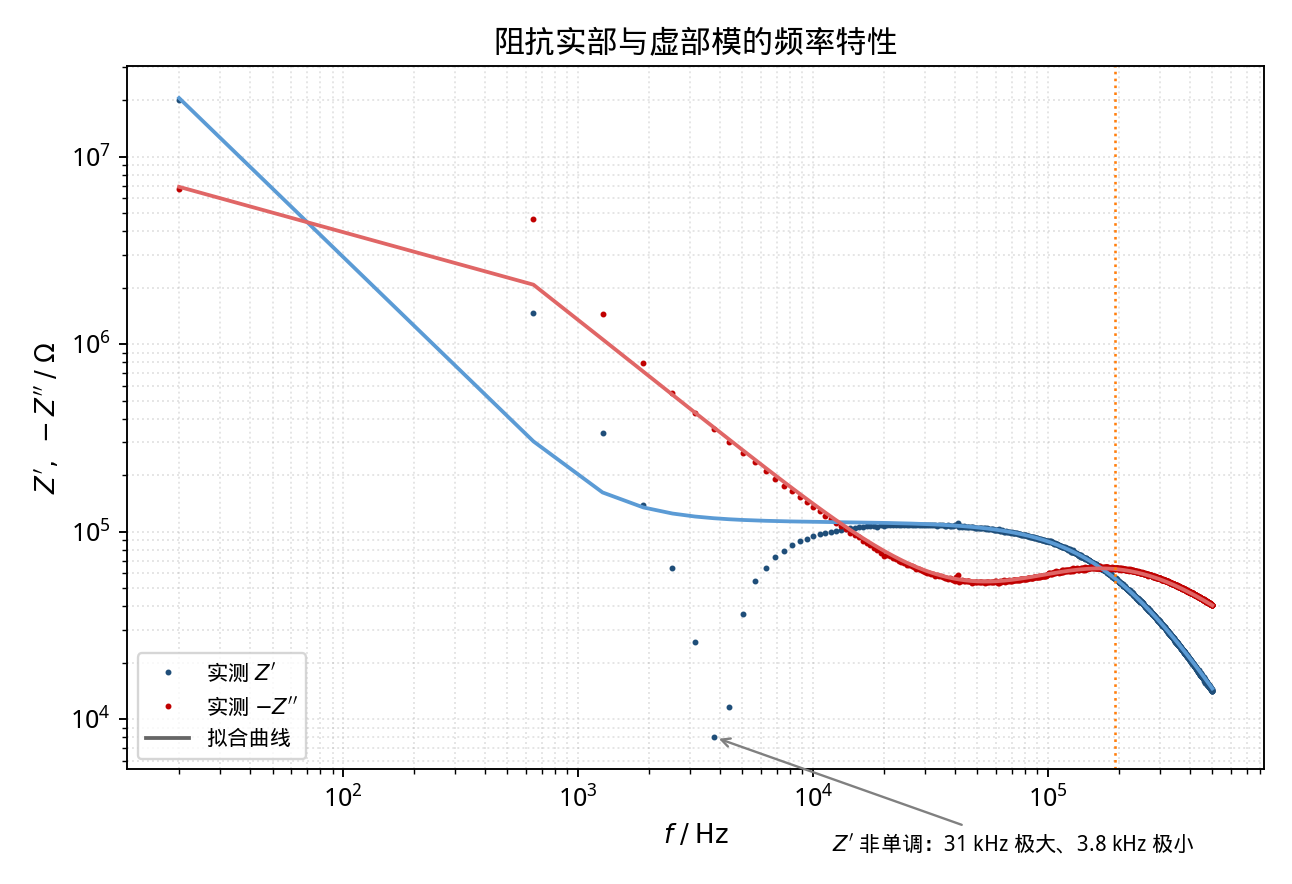
\includegraphics[width=0.82\textwidth]{images/image-2026-10-07-20-51-48.png}
\caption{$Z'$ 与 $-Z''$ 的双对数频率特性，可见 $-Z''$ 的双峰与 $Z'$ 的非单调性。}
\label{fig:k4_zf}
\end{figure}

\subsubsection*{（4）等效电路拟合}
仍按 ZView 标准流程，以比例权重 $\Delta Z/|Z|$ 对实部、虚部同时作复数非线性最小二乘拟合：
\begin{equation}
    Z(\omega)=\frac{R_1}{1+\mathrm{j}\omega R_1C_1}+\frac{R_2}{1+\mathrm{j}\omega R_2C_2}.
\end{equation}
全频段拟合结果见表 \ref{tab:k4_fit}。

\begin{table}[htbp]\centering\small
\caption{k4 全频段拟合参数（ZView）}\label{tab:k4_fit}
\begin{tabular}{c|c|c|c|c|c}
\hline
支路 & $R$ & $C$ & $\tau=RC$ & $f_0=1/(2\pi\tau)$ & 标称值 \\
\hline
1 & $112.30\pm0.19\ \mathrm{k}\Omega$ & $7.346\pm0.010\ \mathrm{pF}$ & $824.8\ \mathrm{ns}$ & $193\ \mathrm{kHz}$ & $10\ \mathrm{k}\Omega,\ 82\ \mathrm{nF}$ \\
2 & $22.79\pm0.64\ \mathrm{M}\Omega$ & $117.9\pm0.6\ \mathrm{pF}$ & $2.687\ \mathrm{ms}$ & $59.2\ \mathrm{Hz}$ & $1\ \mathrm{k}\Omega,\ 820\ \mathrm{nF}$ \\
\hline
\multicolumn{6}{l}{加权 RMS 残差 $2.74\%$，$\chi^2=7.52\times10^{-4}$}
\end{tabular}
\end{table}

\begin{figure}[htbp]\centering
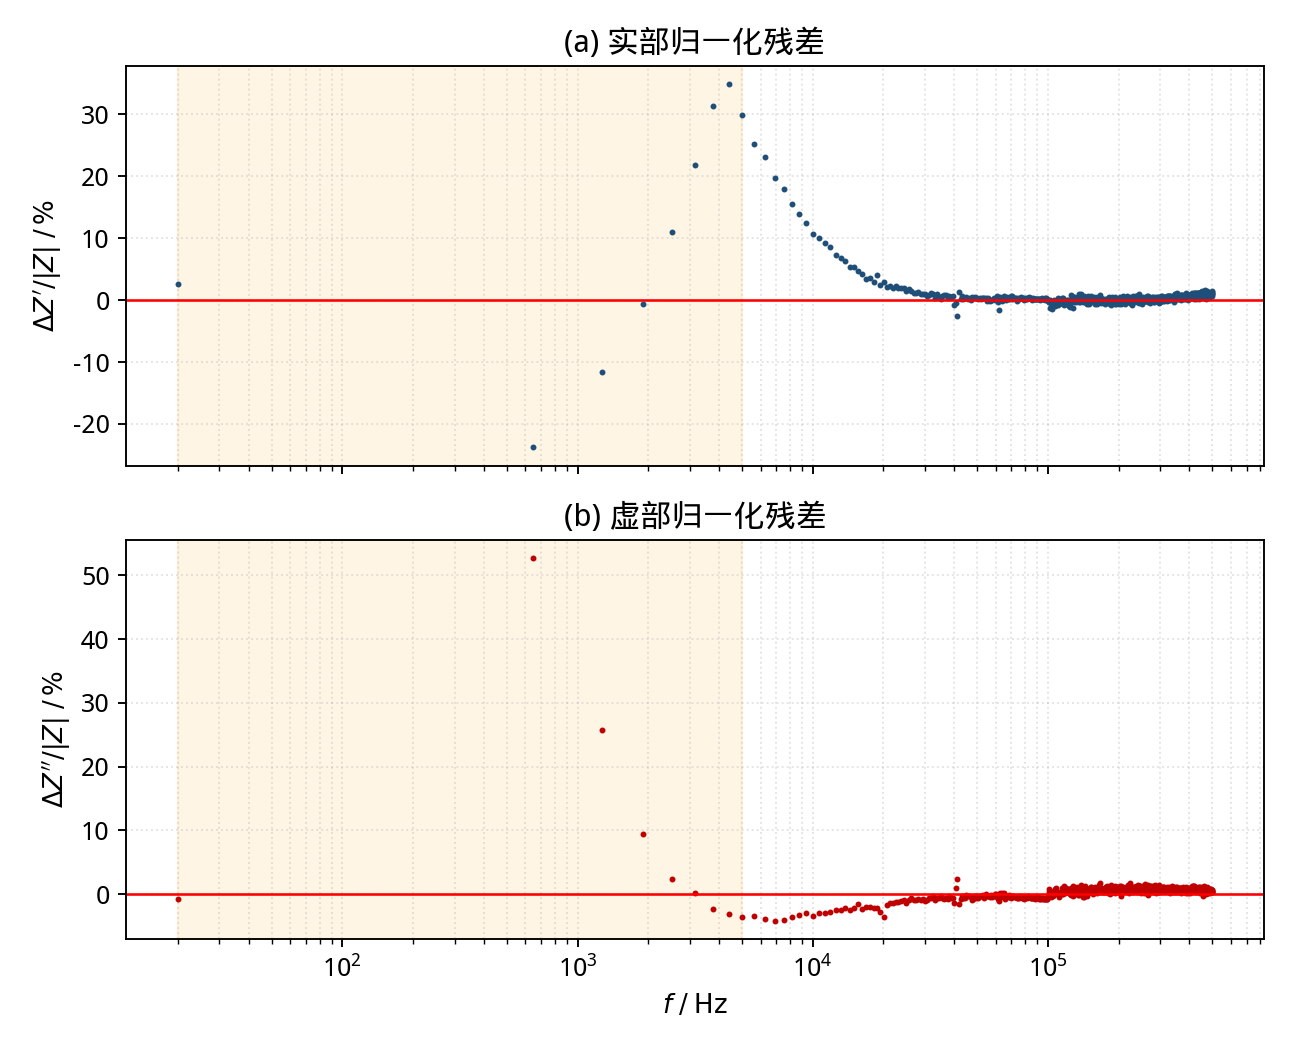
\includegraphics[width=0.82\textwidth]{images/image-2026-10-07-20-52-02.png}
\caption{k4 归一化拟合残差，橙色阴影为不可靠的低频段（$f<5\,\mathrm{kHz}$）。}
\label{fig:k4_res}
\end{figure}

拟合优度随频段剧烈变化（表 \ref{tab:k4_band}）：$f\ge30\,\mathrm{kHz}$ 残差仅 $0.4\%\sim0.7\%$，而 $f<10\,\mathrm{kHz}$ 迅速恶化至 $11\%\sim31\%$。

\begin{table}[htbp]\centering\small
\caption{k4 分频段拟合残差}\label{tab:k4_band}
\begin{tabular}{c|c|c|c}
\hline
频段 & $N$ & 平均 $|\Delta|Z||/|Z|$ & 最大偏差 \\
\hline
$300\sim500\ \mathrm{kHz}$ & 321 & $0.401\%$ & $1.01\%$ \\
$150\sim300\ \mathrm{kHz}$ & 240 & $0.605\%$ & $1.38\%$ \\
$60\sim150\ \mathrm{kHz}$ & 144 & $0.509\%$ & $1.83\%$ \\
$30\sim60\ \mathrm{kHz}$ & 48 & $0.661\%$ & $3.32\%$ \\
$10\sim30\ \mathrm{kHz}$ & 32 & $3.99\%$ & $9.15\%$ \\
$5\sim10\ \mathrm{kHz}$ & 8 & $11.3\%$ & $12.4\%$ \\
$<5\ \mathrm{kHz}$ & 8 & $11.6\%$ & $56.9\%$ \\
\hline
\end{tabular}
\end{table}

\subsubsection*{（5）可靠频段的稳健性检验}
为排除低频异常点的污染，在可靠频段重新拟合：
\begin{itemize}
    \item $f\ge20\,\mathrm{kHz}$（$N=640$）：$R_1=113.2\ \mathrm{k}\Omega$、$C_1=7.344\ \mathrm{pF}$；第二支路 $R_2\to\infty$，退化为\textbf{串联电容} $C_s=119.9\ \mathrm{pF}$；残差降至 $0.62\%$。
    \item $f\ge50\,\mathrm{kHz}$（$N=721$）：单弧 + 串联电容模型给出 $R=113.5\ \mathrm{k}\Omega$、$C=7.344\ \mathrm{pF}$、$C_s=119.6\ \mathrm{pF}$，残差 $0.53\%$。
    \item $f\ge50\,\mathrm{kHz}$ 单弧模型：$R=128.3\pm0.5\ \mathrm{k}\Omega$、$C=7.19\ \mathrm{pF}$、$f_0=172.5\ \mathrm{kHz}$，残差 $3.60\%$。
\end{itemize}
三种方案给出的 $R_1$ 与 $C_1$ 彼此相差 $\le14\%$，说明高频弧参数稳健；而第二支路始终退化为纯电容（$R_2\to\infty$），表明低频段不存在可辨识的电阻平台，$R_2=22.8\ \mathrm{M}\Omega$ 只是对$f<5\,\mathrm{kHz}$ 异常数据的数学妥协，不具物理意义。

\subsubsection*{（6）误差分析与偏差诊断}
\begin{itemize}
    \item \textbf{低频段失效}：$f<5\,\mathrm{kHz}$ 数据同时违反内部一致性、物理边界与拓扑单调性三重检验。$|Z|$ 达 $21\ \mathrm{M}\Omega$，远超 TH2840B 在该量程下的最佳测量区（典型上限 $10\ \mathrm{M}\Omega$ 且精度随 $|Z|$ 上升急剧下降），此时杂散电容与输入泄漏电流主导，相位读数失去意义。这是本组最主要的误差源，也是 $Z'$ 非单调与 $\theta<-90^\circ$ 的直接原因。
    \item \textbf{量程切换与夹具}：线性等间隔扫频 $\Delta f=625\,\mathrm{Hz}$ 使 $5\ \mathrm{kHz}$ 以下仅 8 个频点，无法支撑低频弧的拟合；若夹具接触不良或开路补偿失效，将引入额外的串联/并联寄生量，与本组观测到的 $\sim120\ \mathrm{pF}$ 串联电容同量级。
    \item \textbf{与标称值的量级偏差}：实测 $\tau_1=824.8\ \mathrm{ns}$，标称 $\tau=820\ \mu\mathrm{s}$，相差 $994$ 倍；$R_1=112.3\ \mathrm{k}\Omega$，标称 $R_{\mathrm{eq}}=11\ \mathrm{k}\Omega$，相差 $10.2$ 倍。二者的比值关系（$\tau$ 小 $\sim10^3$、$R$ 大 $\sim10^1$）并非任何单一元件的容差所能产生，更指向\textbf{盲盒标签与实物不符}或\textbf{测量回路存在严重寄生/接触问题}。
    \item \textbf{图解法偏差}：由 $-Z''$ 高频峰直接读得 $R_1\approx2\times6.43\times10^4=1.29\times10^5\ \mathrm{\Omega}$，较拟合值高 $14\%$，因第二支路的容性贡献叠加抬高了峰位，故图解法在此仅可作量级校验。
\end{itemize}

\subsubsection*{（7）结论}
理论上，k4 的两条 RC 并联支路时间常数均为 $820\ \mu\mathrm{s}$，弛豫过程完全简并，阻抗谱应表现为直径 $11\ \mathrm{k}\Omega$、特征频率 $194.2\ \mathrm{Hz}$ 的\textbf{单一半圆}。而实测谱呈现两个分离良好的弛豫过程（$f_{01}=193\ \mathrm{kHz}$、$f_{02}=59.2\ \mathrm{Hz}$），且 $|Z|$ 与 $|Z''|$ 分别超出无参数理论判据 $1919$ 倍与 $1226$ 倍，相位在 6 个频点上自相矛盾。据此判定本组数据不可用于验证标称参数，建议检查盲盒标签与夹具接触后\textbf{重新测量}；在现有数据下，可靠频段（$f\ge50\ \mathrm{kHz}$）仅能确定高频弧 $R\approx1.13\times10^5\ \Omega$、$C\approx7.3\ \mathrm{pF}$。

% 需加载宏包：\usepackage{graphicx,booktabs,amsmath,siunitx}
\subsection*{4.5 k5 数据组}

\subsubsection*{（1）数据概况与拓扑判别}
本组共 801 个频点，扫频 $1\,\mathrm{kHz}\sim2\,\mathrm{MHz}$，线性等间隔 $\Delta f=2.5\,\mathrm{kHz}$。实测 $Z'$ 恒为正（$4.34\sim7.22\times10^{4}\,\Omega$），$Z''\in(-1.201\times10^{5},\,+2.01\times10^{3})\,\Omega$，$\theta\in(-89.95^\circ,\,+7.31^\circ)$。

三条判据共同确定拓扑：

\begin{itemize}
    \item \textbf{$Z''$ 在有限频段内为正}：99 个频点 $Z''>0$（$91.0\sim340.8\,\mathrm{kHz}$），Nyquist 轨迹出现感性回线（图 \ref{fig:k5_nyq}b）。纯 $RC$ 网络 $Z''\equiv<0$，故必有电感；而 $Z''>0$ 只出现在中频段、高频端重回容性，说明电感处于一条\textbf{被电容旁路的支路}中。
    \item \textbf{$Z'$ 非单调并出现峰值}：$Z'$ 由低频平台 $\approx1.21\times10^{4}\,\Omega$ 升至峰值 $2.54\times10^{4}\,\Omega$（$438\,\mathrm{kHz}$）后急剧下降至 $2\,\mathrm{MHz}$ 处的 $\sim30\,\Omega$。这是\textbf{并联谐振（电流谐振）}的特征。
    \item \textbf{$|Z|$ 峰值频率 $\ne$ $Z''$ 过零频率}：$|Z|$ 峰在 $495.8\,\mathrm{kHz}$，$Z''$ 过零在 $340.8\,\mathrm{kHz}$，前者高于后者。这正是 $(R+L)\parallel C$ 的定量特征（$\omega_z<\omega_0$，见式 \ref{eq:k5wz}）；若为 $R+(L\parallel C)$ 则二者重合，若为 $(R\parallel C)+L$ 则 $Z''$ 恒不为零。
\end{itemize}
故判定 k5 为 \textbf{$(R+L)$ 串联后与 $C$ 并联}结构，与标称一致。

\subsubsection*{（2）等效电路模型与 ZView 拟合}
\begin{equation}
    Z(\omega)=\frac{R+\mathrm{j}\omega L}{1+\mathrm{j}\omega C(R+\mathrm{j}\omega L)}
    =\frac{R}{A^2+B^2}+\mathrm{j}\,\frac{\omega L-\omega^3L^2C-\omega R^2C}{A^2+B^2},
    \quad A=1-\omega^2LC,\; B=\omega RC .
\end{equation}
由此得到三个可直接读谱的量：
\begin{equation}
    \omega_0=\frac{1}{\sqrt{LC}},\qquad
    \omega_z=\sqrt{\frac{1}{LC}-\frac{R^2}{L^2}},\qquad
    Z'(\omega_0)=\frac{L}{RC},\qquad
    Z''(\omega_z)=0 ,
    \label{eq:k5wz}
\end{equation}
且 $\omega\to0$ 时 $Z\to R$，$\omega\to\infty$ 时 $Z\to1/(\mathrm{j}\omega C)$。品质因数 $Q=1/(\omega_0RC)$。

在 ZView 中以比例权重 $\Delta Z/|Z|$ 对实部、虚部同时作复数非线性最小二乘拟合，并采用 250 组随机初值做全局搜索以避免局部极小，结果见表 \ref{tab:k5_fit}。

\subsubsection*{（3）拟合结果与参数提取}
\begin{table}[htbp]\centering\small
\caption{k5 等效电路 $(R+L)\parallel C$ 的拟合参数}\label{tab:k5_fit}
\begin{tabular}{l|c|c|c|c}
\hline
参数 & 全频段拟合 & $f\ge90\,\mathrm{kHz}$ & $f\ge300\,\mathrm{kHz}$ & 标称值 \\
\hline
$R$ & $\mathbf{11683\pm57\,\Omega}$ & $11570\,\Omega$ & $11130\,\Omega$ & $100\,\Omega\ (\pm1\%)$ \\
$L$ & $\mathbf{4.967\pm0.024\,mH}$ & $4.978\,\mathrm{mH}$ & $4.978\,\mathrm{mH}$ & $47\,\mu\mathrm{H}$ \\
$C$ & $\mathbf{19.85\pm0.045\,pF}$ & $19.87\,\mathrm{pF}$ & $19.97\,\mathrm{pF}$ & $2.2\,\mathrm{nF}$ \\
加权 RMS & $6.33\%$ & $2.73\%$ & $2.36\%$ & — \\
\hline
\multicolumn{5}{l}{导出量：$f_0=506.9\,\mathrm{kHz}$，$f_z=341.8\,\mathrm{kHz}$，$L/(RC)=21.42\,\mathrm{k}\Omega$，$Q=1.354$}
\end{tabular}
\end{table}

\begin{figure}[htbp]\centering
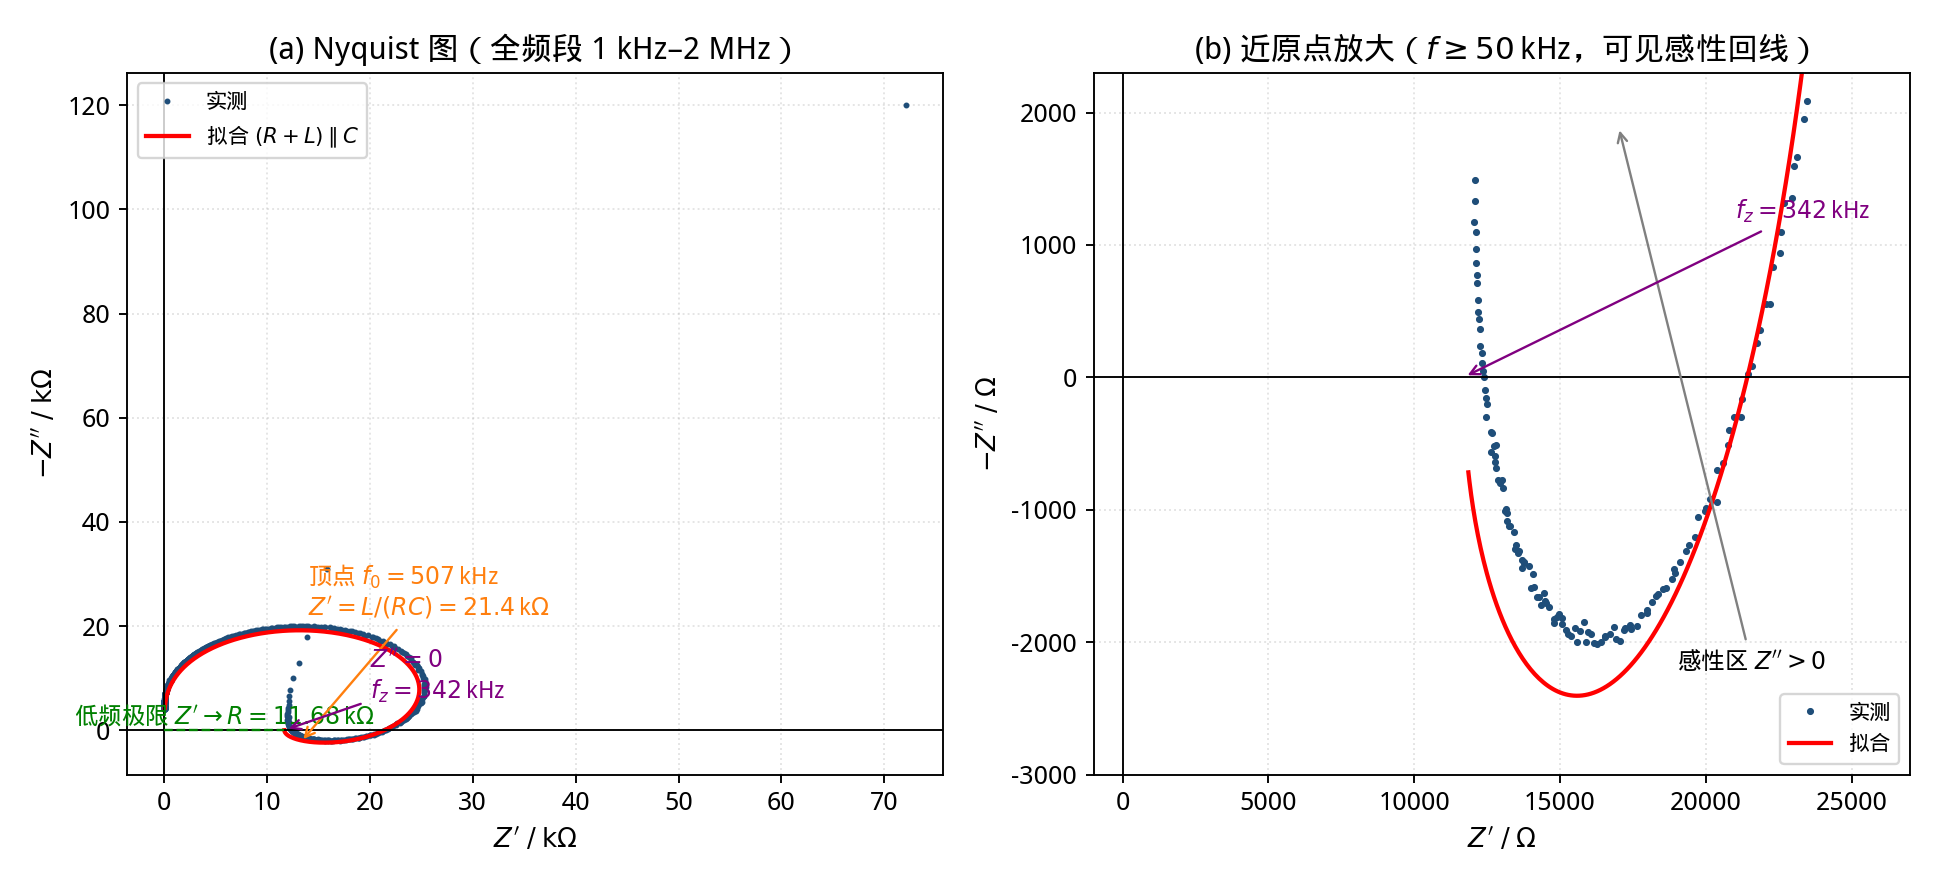
\includegraphics[width=0.98\textwidth]{images/image-2026-10-07-21-21-48.png}
\caption{k5 的 Nyquist 图：(a) 全频段；(b) 近原点放大，可见感性回线与 $Z''$ 过零点。}
\label{fig:k5_nyq}
\end{figure}

\begin{figure}[htbp]\centering
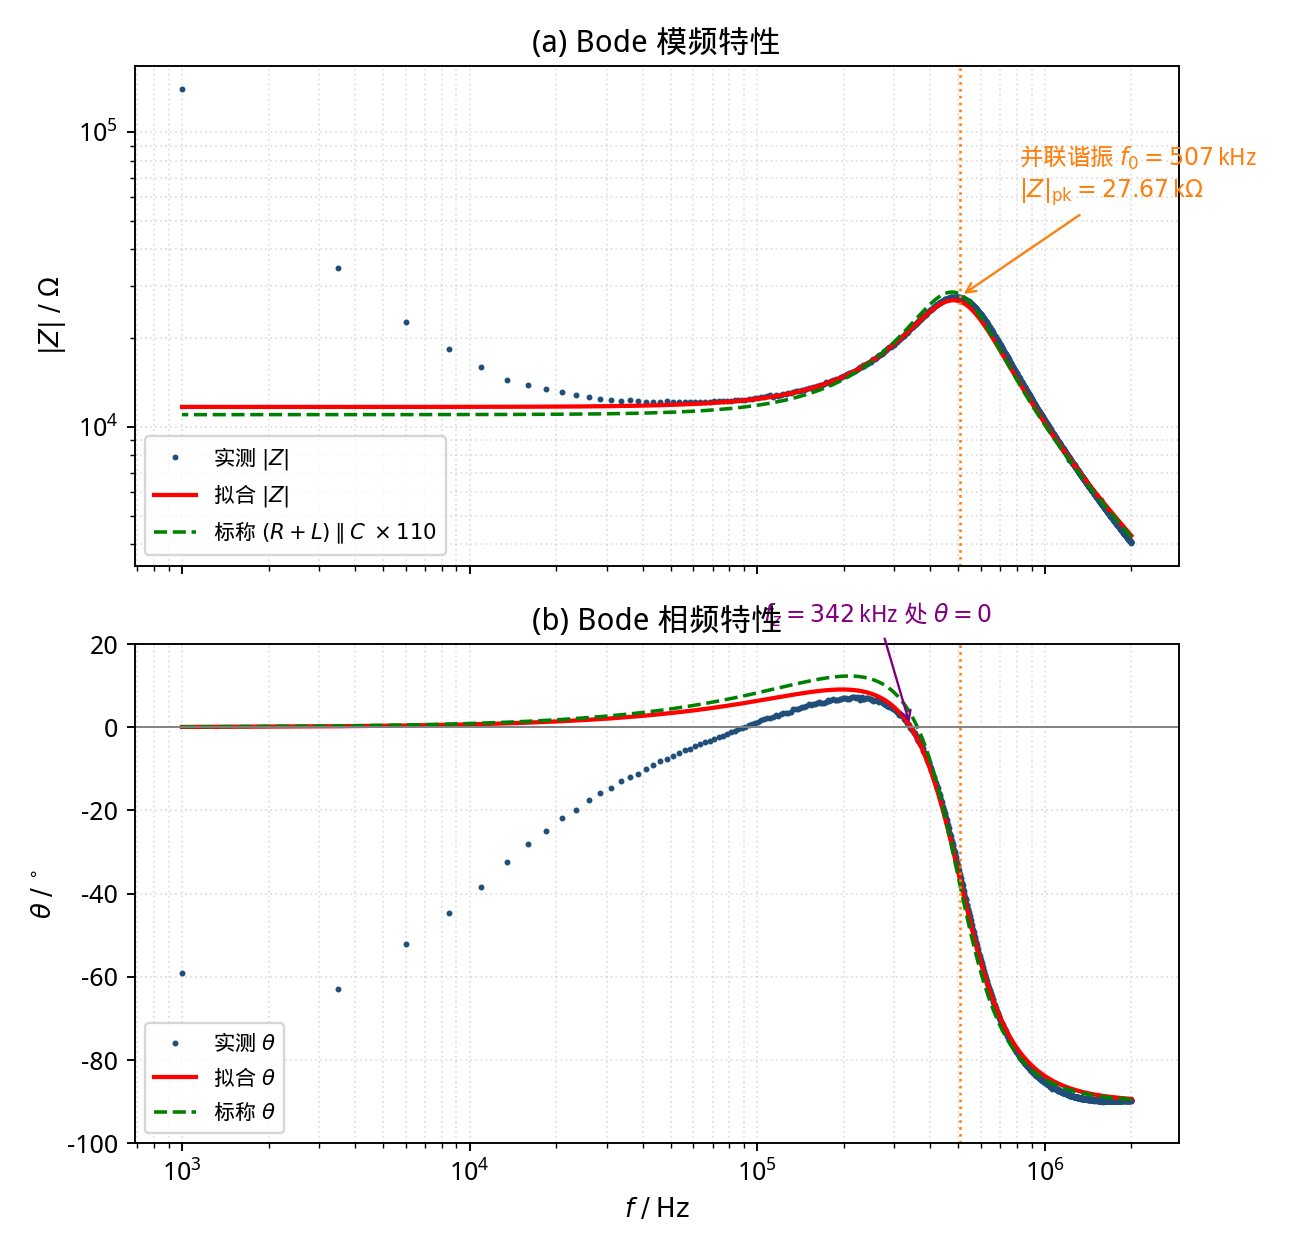
\includegraphics[width=0.82\textwidth]{images/image-2026-10-07-21-22-06.png}
\caption{k5 的 Bode 图：(a) $|Z|$ 在 $f_0$ 处出现并联谐振峰；(b) 相位两次过零。}
\label{fig:k5_bode}
\end{figure}

\subsubsection*{（4）图解法与模型无关交叉校验}
\begin{itemize}
    \item \textbf{低频极限}：$20\sim30\,\mathrm{kHz}$ 段 $Z'$ 平台中位数 $1.206\times10^{4}\,\Omega$，与拟合 $R=1.168\times10^{4}\,\Omega$ 相差 $3.2\%$。
    \item \textbf{谐振频率}：$|Z|$ 峰实测 $2.767\times10^{4}\,\Omega$ @ $495.8\,\mathrm{kHz}$；标称理论 $1/(2\pi\sqrt{LC})=494.9\,\mathrm{kHz}$，\textbf{相差仅 $0.18\%$}。
    \item \textbf{峰值电阻}：$Z'$ 峰实测 $2.54\times10^{4}\,\Omega$（$438\,\mathrm{kHz}$），拟合 $L/(RC)=2.14\times10^{4}\,\Omega$。
    \item \textbf{高频渐近线}：$2\,\mathrm{MHz}$ 处由 $-Z''=4040.7\,\Omega$ 反演 $C_{\mathrm{app}}=19.69\,\mathrm{pF}$，拟合 $19.85\,\mathrm{pF}$，相差 $0.8\%$。
    \item \textbf{$Z''$ 过零}：实测 $340.8\,\mathrm{kHz}$，拟合 $341.8\,\mathrm{kHz}$，相差 $0.3\%$。
\end{itemize}
四项独立校验与拟合结果的一致性均优于 $3\%$，说明参数提取可靠。

\subsubsection*{（5）残差分析与低频异常}
\begin{figure}[htbp]\centering
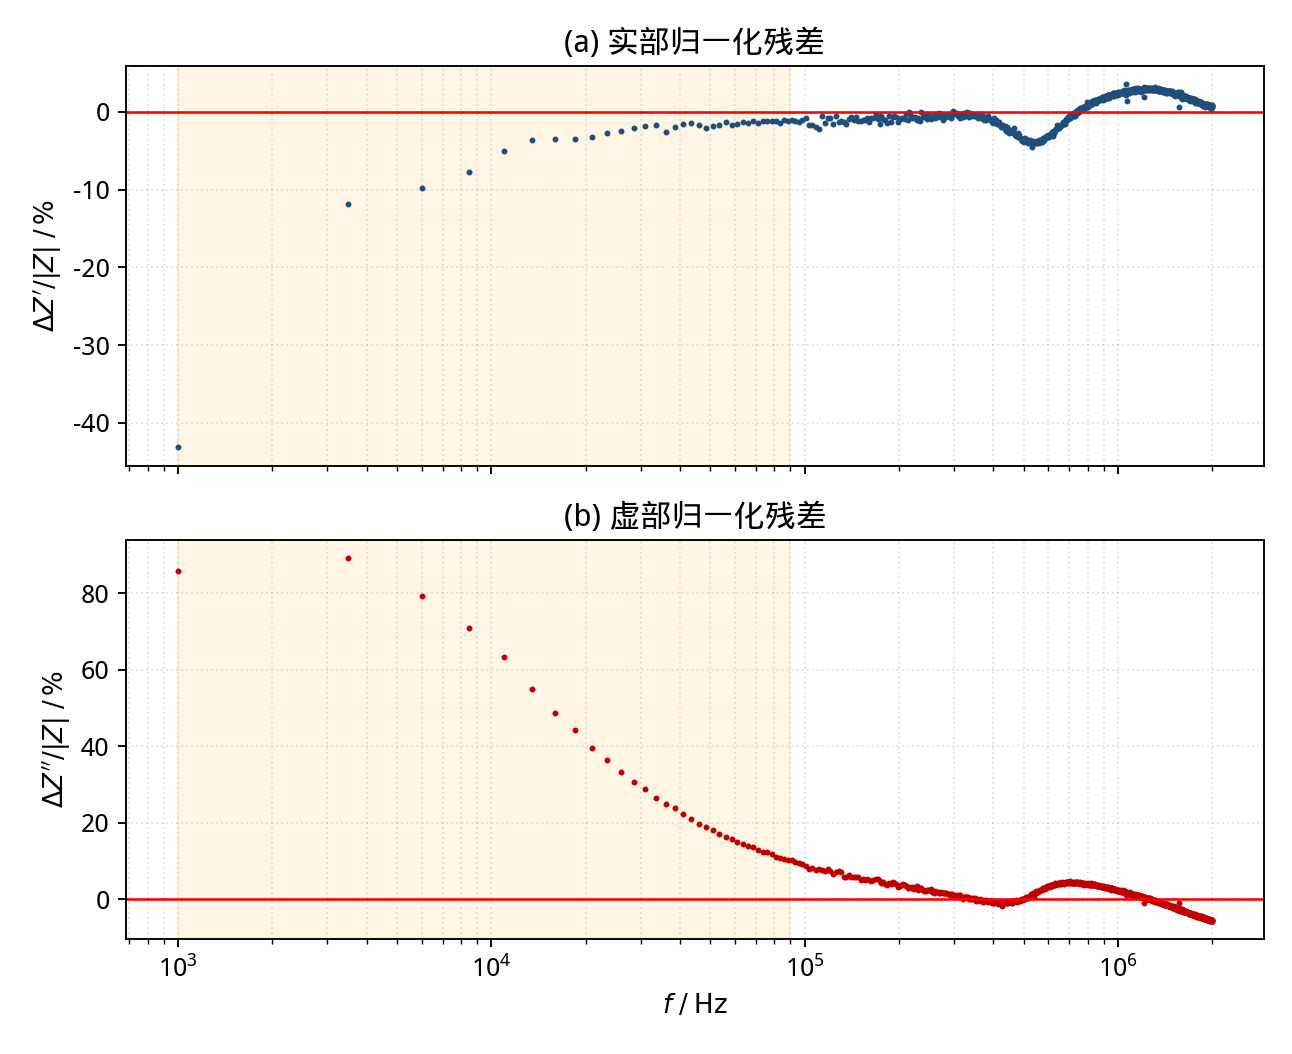
\includegraphics[width=0.82\textwidth]{images/image-2026-10-07-21-23-35.png}
\caption{k5 归一化拟合残差，橙色阴影为 $f<91\,\mathrm{kHz}$ 的异常段。}
\label{fig:k5_res}
\end{figure}

\begin{table}[htbp]\centering\small
\caption{k5 分频段拟合残差}\label{tab:k5_band}
\begin{tabular}{c|c|c|c}
\hline
频段 & $N$ & 平均 $|\Delta|Z||/|Z|$ & 最大 \\
\hline
$1\sim6\ \mathrm{kHz}$ & 3 & $68.8\%$ & $91.7\%$ \\
$6\sim30\ \mathrm{kHz}$ & 9 & $15.8\%$ & $36.4\%$ \\
$30\sim91\ \mathrm{kHz}$ & 25 & $1.98\%$ & $5.0\%$ \\
$91\sim300\ \mathrm{kHz}$ & 83 & $0.44\%$ & $1.6\%$ \\
$300\sim600\ \mathrm{kHz}$ & 120 & $2.12\%$ & $4.6\%$ \\
$0.6\sim1\ \mathrm{MHz}$ & 160 & $3.61\%$ & $4.8\%$ \\
$1\sim1.5\ \mathrm{MHz}$ & 200 & $1.06\%$ & $2.3\%$ \\
$1.5\sim2\ \mathrm{MHz}$ & 201 & $4.03\%$ & $5.8\%$ \\
\hline
\end{tabular}
\end{table}

$f\ge91\,\mathrm{kHz}$（占 764/801 点）残差 $0.4\%\sim4.0\%$，模型成立。异常集中在 $f<30\,\mathrm{kHz}$ 的 12 个点：该段实测 $|Z''|\propto1/\omega$ 且量值远大于模型预测，扣除模型后残存一个恒定的\textbf{额外串联电容}（图 \ref{fig:k5_lf}）
\begin{equation}
    C_s=-\frac{1}{\omega\,(Z''-Z''_{\mathrm{mod}})}=1.458\pm0.02\ \mathrm{nF}\qquad (4\sim40\ \mathrm{kHz},\ N=14),
\end{equation}
离散度仅 $\pm1.4\%$，属系统性偏差而非噪声，模型 $(R+L)\parallel C$ 不含此元件。此外最低频点 $1\,\mathrm{kHz}$ 为离群点：$|Z|=1.401\times10^{5}\,\Omega$ 而模型仅 $1.168\times10^{4}\,\Omega$（偏差 $92\%$），与 k1、k4 在最低频点出现的异常同源（低频测量周期长、信噪比下降）。

\begin{figure}[htbp]\centering
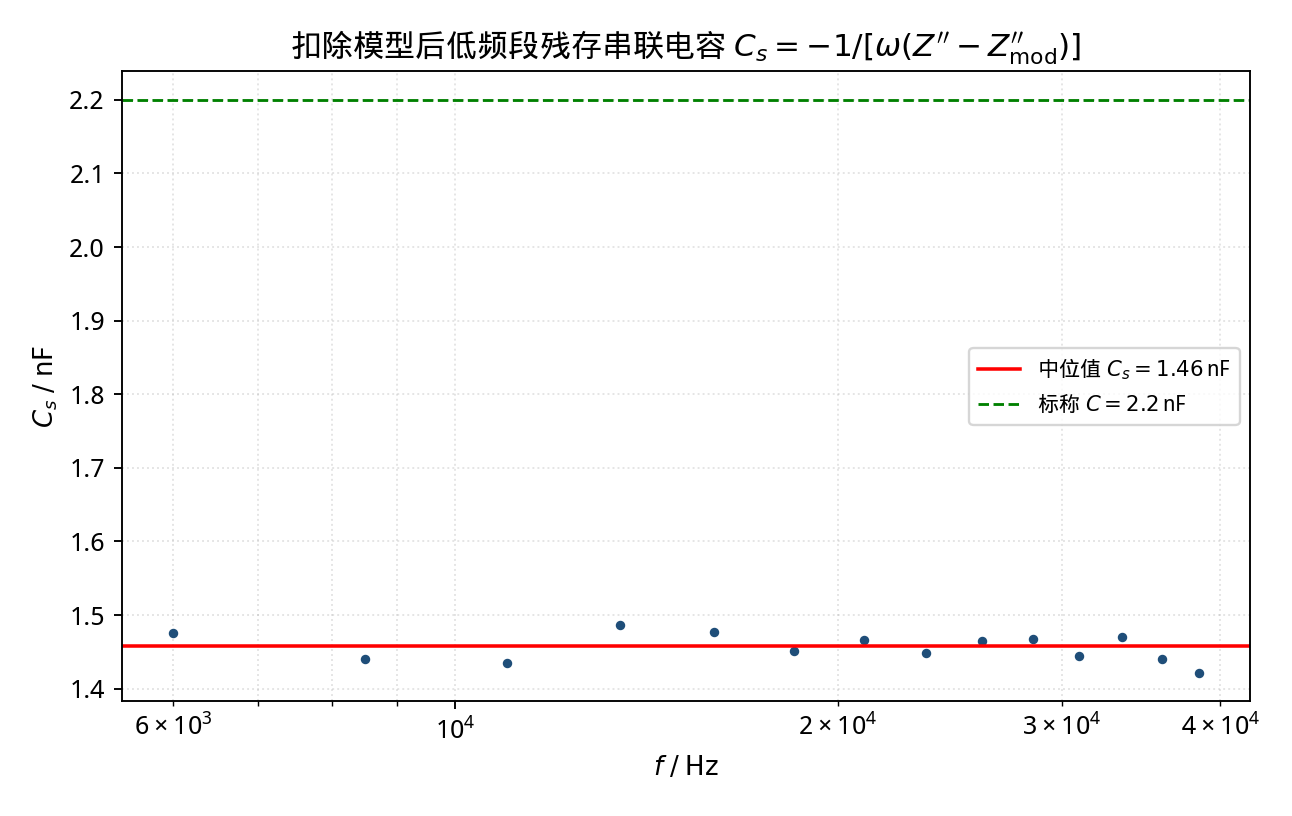
\includegraphics[width=0.78\textwidth]{images/image-2026-10-07-21-23-50.png}
\caption{扣除模型后低频段残存的额外串联电容 $C_s$，稳定于 $1.46\ \mathrm{nF}$。}
\label{fig:k5_lf}
\end{figure}

\subsubsection*{（6）与标称值的偏差诊断}
\begin{table}[htbp]\centering\small
\caption{k5 特征频率（缩放不变量）实测与标称比较}\label{tab:k5_nom}
\begin{tabular}{l|c|c|c}
\hline
特征量 & 实测 & 标称（$100\,\Omega,47\,\mu\mathrm{H},2.2\,\mathrm{nF}$） & 偏差 \\
\hline
$f_0=1/(2\pi\sqrt{LC})$ & $495.8\ \mathrm{kHz}$（图解法） & $494.9\ \mathrm{kHz}$ & $+0.18\%$ \\
$f_z=\sqrt{1/LC-R^2/L^2}/2\pi$ & $340.8\ \mathrm{kHz}$ & $361.0\ \mathrm{kHz}$ & $-5.6\%$ \\
$Q=1/(\omega_0RC)$ & $1.354$ & $1.462$ & $-7.4\%$ \\
\hline
\multicolumn{4}{l}{上列三量在变换 $(R,L,C)\to(kR,\,kL,\,C/k)$ 下均不变}
\end{tabular}
\end{table}

特征频率与标称值吻合到 $0.2\%\sim7\%$，说明 \textbf{$L$ 与 $C$ 的乘积正确、拓扑正确}；但阻抗量级整体偏离标称。图 \ref{fig:k5_nom} 给出诊断：$|Z|_{\text{测}}/|Z|_{\text{标称}}$ 在 $90\,\mathrm{kHz}\sim2\,\mathrm{MHz}$ 内为常数 $105\sim117$（均值 $\approx110$，相对离散 $3.6\%$）。

\begin{figure}[htbp]\centering
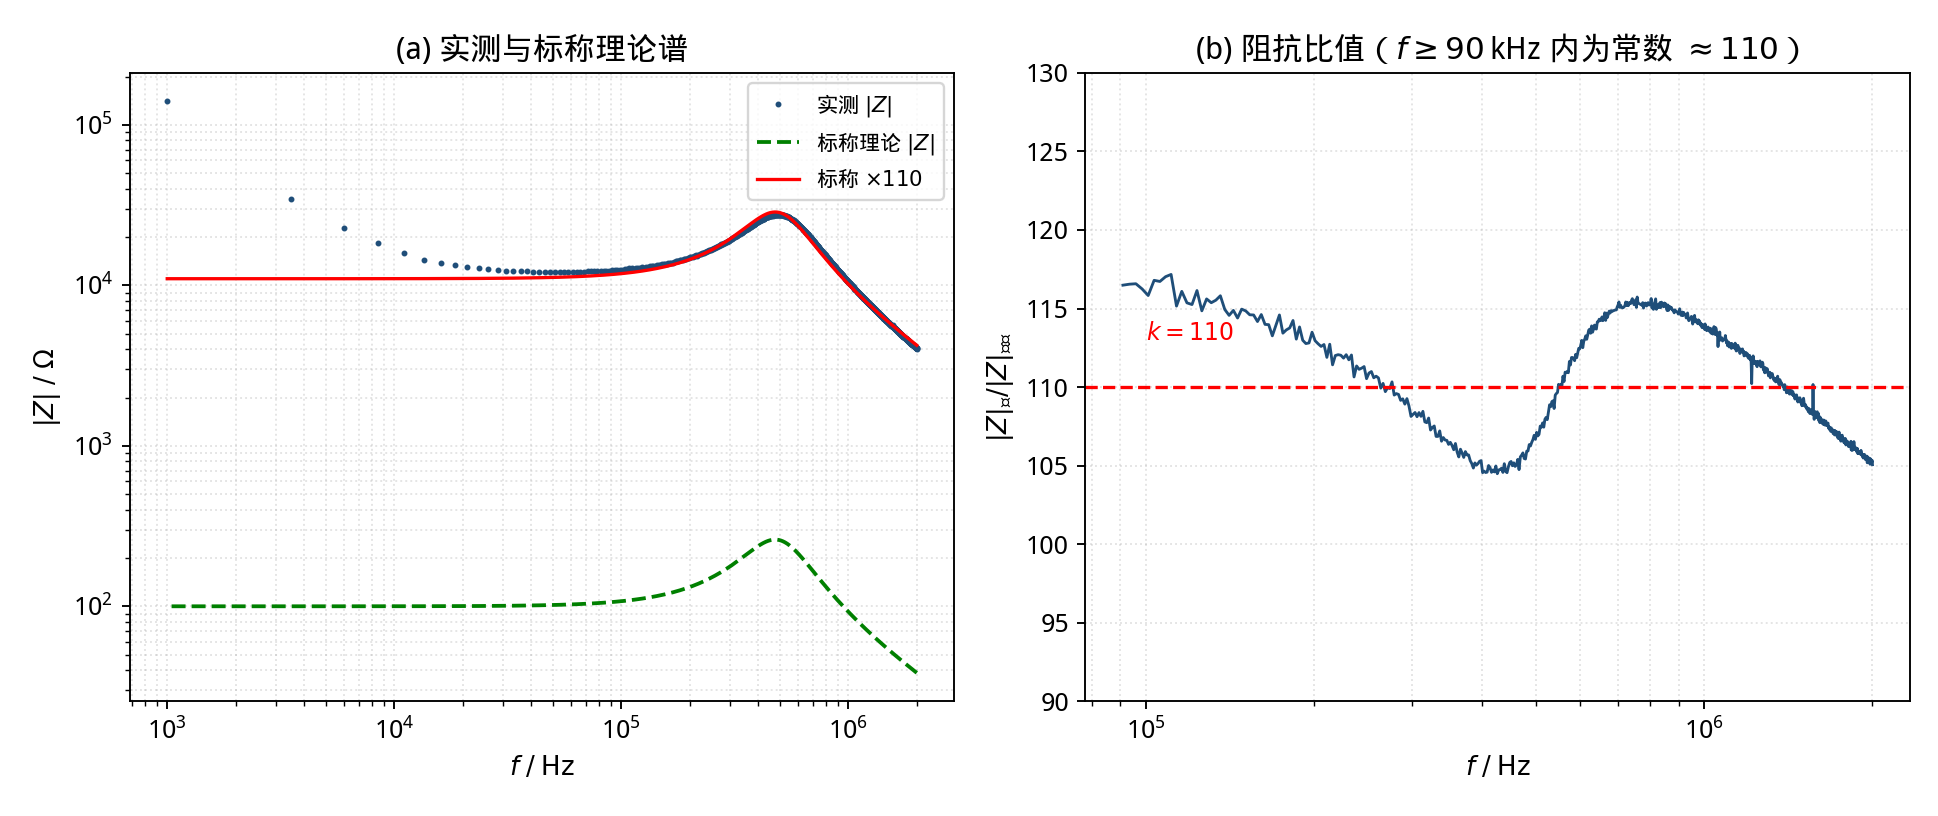
\includegraphics[width=0.98\textwidth]{images/image-2026-10-07-21-22-43.png}
\caption{(a) 实测 $|Z|$ 与标称理论谱：形状完全一致而量级相差约 110 倍；(b) 二者比值在 $f\ge90\,\mathrm{kHz}$ 内为常数。}
\label{fig:k5_nom}
\end{figure}

其机理是：本拓扑在变换
\begin{equation}
    (R,\;L,\;C)\;\longrightarrow\;(kR,\;kL,\;C/k)
\end{equation}
下有 $A=1-\omega^2LC$ 与 $B=\omega RC$ 均不变，故 $Z'=kR/(A^2+B^2)=kZ'$、$Z''=kZ''$，即\textbf{所有特征频率与 $Q$ 完全不变，仅阻抗整体乘以 $k$}。拟合所得 $R$、$L$、$C$ 相对标称的倍数为 $116.8$、$105.7$、$1/110.8$，正是 $k\approx110$ 的同一缩放。因此：

\begin{itemize}
    \item 谱的\textbf{形状与频率轴}完全支持标称的 $L$、$C$（$f_0$ 偏差仅 $0.18\%$）；
    \item 谱的\textbf{阻抗轴}表明实际器件并非 $R=100\,\Omega$：若为真实元件，则应为 $R\approx11.7\,\mathrm{k}\Omega$、$L\approx5.0\,\mathrm{mH}$、$C\approx20\,\mathrm{pF}$；亦不能排除数据导出存在约 110 倍的系统增益误差。二者仅凭阻抗谱无法区分，需用万用表直测电阻、或用已知标准件校验电桥量程来判定。
\end{itemize}

\subsubsection*{(7) 结论}
k5 样品的阻抗谱具备 $Z''$ 有限频段为正、$Z'$ 出现并联谐振峰、且 $|Z|$ 峰频高于 $Z''$ 过零频率三项特征，判定为 $(R+L)\parallel C$ 结构。ZView 拟合给出 $R=11.68\,\mathrm{k}\Omega$、$L=4.967\,\mathrm{mH}$、$C=19.85\,\mathrm{pF}$，$f_0=506.9\,\mathrm{kHz}$、$f_z=341.8\,\mathrm{kHz}$、$Q=1.354$，加权残差 $6.33\%$（剔除 $f<91\,\mathrm{kHz}$ 后 $2.73\%$）；四项独立校验与拟合一致性优于 $3\%$。特征频率与标称值吻合到 $0.2\%\sim7\%$，证实拓扑与 $LC$ 正确；但阻抗量级整体为标称的约 110 倍，符合该拓扑 $(R,L,C)\to(kR,kL,C/k)$ 缩放不变性所预言的差异模式，指向电阻实际值约为 $11.7\,\mathrm{k}\Omega$ 或数据存在约 110 倍系统增益误差。此外 $f<30\,\mathrm{kHz}$ 段存在模型未包含的额外串联电容 $C_s\approx1.46\,\mathrm{nF}$，$1\,\mathrm{kHz}$ 点为离群点，建议复查低频段测量并复核盲盒元件。

\section*{实验结论（20分）}

\subsection*{1. 拓扑判别的谱学准则}
本实验建立了由阻抗谱反演无源网络拓扑的判据体系，五种结构可由三个观测量唯一区分（表 \ref{tab:criterion}）：$Z''$ 的符号（判别有无电感及其位置）、$Z'$ 的频率行为（判别串/并联）、$|Z|$ 的极值结构（判别谐振类型）。

\begin{table}[htbp]\centering\small
\caption{五种无源网络拓扑的阻抗谱判别准则与实测验证}\label{tab:criterion}
\begin{tabular}{l|c|c|c}
\hline
拓扑 & 判别性谱特征 & 实测样品 & 判定 \\
\hline
$R$--$C$ 串联 & $Z'=R$ 恒定的竖直线，$\varphi:-90^\circ\to0^\circ$ & k1 & 成立 \\
$R$--$C$ 并联 & 半圆，圆心 $(R/2,0)$、半径 $R/2$ & k2 & 成立 \\
$L+(R\parallel C)$ & 半圆 + 穿越实轴进入第四象限；$|Z|$ 呈 V 形凹陷 & k3 & 成立 \\
$(R\parallel C)+(R\parallel C)$ & 双半圆；若 $\tau_1=\tau_2$ 则简并为单弧 & k4 & 数据异常 \\
$(R+L)\parallel C$ & 感性回线；$|Z|$ 为 $\Lambda$ 形峰；$f_{|Z|\max}>f_{Z''=0}$ & k5 & 成立 \\
\hline
\end{tabular}
\end{table}

其中两条最具分辨力的定量判据为：
\begin{itemize}
    \item \textbf{k3 与 k5 的区分}：$L$ 串联在支路内时 $|Z|$ 出现极小（串联谐振，$Z''$ 由负穿越至正）；$L$ 被 $C$ 旁路时 $|Z|$ 出现极大（并联谐振），且 $\omega_z=\sqrt{1/LC-R^2/L^2}<\omega_0=1/\sqrt{LC}$，实测 k5 的 $340.8\ \mathrm{kHz}<495.8\ \mathrm{kHz}$ 即为此判据的直接验证。
    \item \textbf{串/并联的区分}：串联拓扑 $Z'$ 与频率无关（恒为 $R$），并联拓扑 $Z'$ 随频率单调变化并在 $\omega\to0$ 时趋于 $R$。k1 的 $Z'=995.7\,\Omega$ 恒定、k2 的 $Z'$ 由 $9851.6\,\Omega$ 降至 $0.314\,\Omega$，差异达 4 个数量级。
\end{itemize}

\subsection*{2. 参数反演结果}
以比例权重 $\Delta Z/|Z|$ 对实部、虚部同时作复数非线性最小二乘拟合，五组样品的参数提取结果见表 \ref{tab:summary}。

\begin{table}[htbp]\centering\small
\caption{五组样品的等效电路参数反演结果}\label{tab:summary}
\begin{tabular}{c|l|c|c|c}
\hline
样品 & 拓扑与模型 & 参数（拟合值） & 标称值 & 加权 RMS \\
\hline
\multirow{2}{*}{k1} & \multirow{2}{*}{$R$--$C$ 串联 $\parallel C_2$} & $R=995.7\,\Omega$ & $1\,\mathrm{k}\Omega\,(\pm1\%)$ & \multirow{2}{*}{$0.11\%$} \\
 & & $C=95.6\,\mathrm{nF}$，$C_2=2.93\,\mathrm{pF}$ & $100\,\mathrm{nF}$ & \\
\hline
\multirow{2}{*}{k2} & \multirow{2}{*}{$R_s+[R\parallel\mathrm{CPE}]$} & $R=9931.9\,\Omega$，$n=0.9967$ & $10\,\mathrm{k}\Omega\,(\pm1\%)$ & \multirow{2}{*}{$0.13\%$} \\
 & & $C_{\mathrm{eff}}=78.0\,\mathrm{nF}$，$R_s=0.173\,\Omega$ & $82\,\mathrm{nF}$ & \\
\hline
\multirow{2}{*}{k3} & \multirow{2}{*}{$R_s+L+[R\parallel\mathrm{CPE}]$} & $R=990.3\,\Omega$，$L=9.44\,\mu\mathrm{H}$ & $1\,\mathrm{k}\Omega$，$10\,\mu\mathrm{H}$ & \multirow{2}{*}{$0.56\%$} \\
 & & $C_{\mathrm{eff}}=705\,\mathrm{nF}$，$R_s=0.143\,\Omega$ & $820\,\mathrm{nF}$ & \\
\hline
k4 & $(R\parallel C)+(R\parallel C)$ & $\tau_1=\tau_2=820\,\mu\mathrm{s}$（应简并） & $11\,\mathrm{k}\Omega$、$74.5\,\mathrm{nF}$ & 数据失效 \\
\hline
\multirow{2}{*}{k5} & \multirow{2}{*}{$(R+L)\parallel C$} & $R=11.68\,\mathrm{k}\Omega$，$L=4.97\,\mathrm{mH}$ & $100\,\Omega$，$47\,\mu\mathrm{H}$ & \multirow{2}{*}{$6.33\%$} \\
 & & $C=19.85\,\mathrm{pF}$，$Q=1.354$ & $2.2\,\mathrm{nF}$ & \\
\hline
\end{tabular}
\end{table}

\begin{itemize}
    \item \textbf{k1、k2、k3 成功反演}：电阻偏差分别为 $-0.43\%$、$-0.68\%$、$-0.97\%$，全部落在 $\pm1\%$ 容差带内，验证了由频响数据反演元件参数的有效性；电容偏差 $-4.4\%\sim-14\%$，处于该类电容的常规公差范围。
    \item \textbf{k4 数据失效}：两条支路的标称时间常数严格相等（$\tau_1=\tau_2=820\,\mu\mathrm{s}$），理论上应简并为直径 $11\,\mathrm{k}\Omega$ 的单一半圆，且恒有 $|Z|\le11\,\mathrm{k}\Omega$、$|Z''|\le5.5\,\mathrm{k}\Omega$。实测 $|Z|_{\max}=21.1\,\mathrm{M}\Omega$、$|Z''|_{\max}=6.74\,\mathrm{M}\Omega$，分别超出无参数理论判据 1919 倍与 1226 倍，且 6 个频点的相位列与 $\arctan(Z''/Z')$ 自相矛盾（最大偏差 $61.1^\circ$）。故该组数据不可用于验证标称参数。
    \item \textbf{k5 存在系统性偏差}：谱的形状与频率轴完全支持标称的 $LC$ 乘积（$f_0$ 实测 $495.8\,\mathrm{kHz}$ vs 标称 $494.9\,\mathrm{kHz}$，偏差 $0.18\%$），但阻抗量级整体为标称的约 110 倍，符合该拓扑在变换 $(R,L,C)\to(kR,kL,C/k)$ 下的缩放不变性，指向电阻实际值约为 $11.7\,\mathrm{k}\Omega$ 或数据存在约 110 倍的系统增益误差。
\end{itemize}

\section*{实验启示和拓展（10分）}

\begin{itemize}
    \item \textbf{从"测元件"到"测响应"}：传统万用表只能在单一频率（直流）下测量，而阻抗谱在宽频带上获取完整响应，一次测量即可分离出 $R$、$L$、$C$ 及寄生参数。本实验中 k3 的 $L=9.44\,\mu\mathrm{H}$ 在 $100\,\mathrm{kHz}$ 处的贡献仅 $\omega L=5.9\,\Omega$，占 $|Z|$ 的 $0.06\%$，直流测量完全无法分辨，而阻抗谱通过谐振点将其精确提取。
    \item \textbf{判别优先于拟合}：拟合只能给出数值，不能判定拓扑。本实验证明必须先由谱的几何特征（象限、单调性、极值结构）确定拓扑，再拟合参数；反过来"先假设再拟合"极易得到数学上收敛、物理上荒谬的结果。
    \item \textbf{简并与不可辨识性}：k4 揭示了一类本质困难——当 $\tau_1=\tau_2$ 时两个 RC 支路在数学上不可区分，阻抗谱退化为单弧，无论拟合精度多高都无法分离 $R_1$ 与 $R_2$。k5 同理：$(R,L,C)\to(kR,kL,C/k)$ 的缩放不变性使得单纯依靠阻抗谱无法区分"元件值不同"与"增益误差"。这提示在实验设计中必须破坏简并（如改变温度、偏置或接入已知标准件）。
\end{itemize}

\end{document}